%\documentclass[11pt,a4paper]{article}
\documentclass[11pt
  , a4paper
  , article
  , oneside
%  , twoside
%  , draft
]{memoir}

\usepackage{control}
\usepackage[numbers]{natbib}
\usepackage{hyperref}

\begin{document}

\newcommand{\technumber}{
  RAON Control-Document Series\\
  Revision : v0.4,   Release : 2016. 01. 06}
\title{\textbf{Manual for Archiver Appliance}}


\author{Seung Hee Nam\thanks{namsh@ibs.re.kr} \\
  Control Group \\
  Rare Isotope Science Project\\
  Institute for Basic Science\\
  Daejeon, South Korea
}

\date{\today}

\renewcommand{\maketitlehooka}{\begin{flushright}\textsf{\technumber}\end{flushright}}
%\renewcommand{\maketitlehookb}{\centering\textsf{\subtitle}}
%\renewcommand{\maketitlehookc}{C}
%\renewcommand{\maketitlehookd}{D}

\maketitle

\begin{abstract}
 Archiver Appliance was developed by Stanford Linear Accelerator Center (SLAC) national laboratory of the United States. RISP (Rare Isotope Science Project) control system use the archiver appliance and to customize RISP enviroment. This document include archiver appliance quickstart guide and installation guide. If you want to simply test the system and quickly get going, please see the quickstart section. If you plan to have only one machine in your site, you can consider using the install script that comes with the installation bundle. This install script accommodates installations with a "standard" set of parameters and installs the EPICS archiver appliance on one machine.
\end{abstract}



\chapter{EPICS Base Installation}

\section{About EPICS}
EPICS\cite{epics} is a set of software tools and applications which provide a software infrastructure for use in building distributed control systems to operate devices such as Particle Accelerators, Large Experiments and major Telescopes. Such distributed control systems typically comprise tens or even hundreds of computers, networked together to allow communication between them and to provide control and feedback of the various parts of the device from a central control room, or even remotely over the internet.
If you want to learn more about EPICS, a good place to start is the \href{http://www.aps.anl.gov/epics/docs/GSWE.php}{Getting Started with EPICS }lecture series which provides online videos of a series of lectures presented at Argonne in 2004-2005.
\section{License}
EPICS is provided under an open source license called the EPICS Open License, which is similar to the BSD license. See the \href{http://www.aps.anl.gov/epics/license/index.php}{Licensing} pages for details and some history.
\section{System requirements}
\subsection{GNU make}
You must use GNU make, gnumake, for any EPICS builds. Set your path so that a gnumake version 3.81 or later is available.
\subsection{Perl}
You must have Perl version 5.8.1 or later installed. The EPICS configuration files do not specify the perl full pathname, so the perl executable must be found through your normal search path.
\subsection{Unzip and tar (Winzip on WIN32 systems)}
You must have tools available to unzip and untar the EPICS base distribution file.
\subsection{GNU readline or Tecla library}
GNU readline and Tecla librararies can be used by the IOC shell to provide command line editing and command line history recall and edit. GNU readline (or Tecla library) must be installed on your target system when COMMANDLINE\_LIBRARY is set to READLINE (or TECLA) for that target. EPICS (EPICS shell) is the default specified in CONFIG\_COMMON. A READLINE override is defined for linux-x86 in the EPICS distribution. Comment out COMMANDLINE\_LIBRARY=READLINE in configure/os/CONFIG\_SITE.Common.linux\-x86 if readline is not installed on linux\-x86. Command\-line editing and history will then be those supplied by the os. On vxWorks the ledLib command-line input library is used instead.
\subsection{Tip}
Here is the quick installation log for Debian Linux user. Other Linux users install the same name package. 
\begin{itemize}
	\item GNU make
\begin{lstlisting}[style=termstyle]
	Package: build-essential
	ex> root@user:~$ aptitude install build-essential
\end{lstlisting}
	\item Perl
\begin{lstlisting}[style=termstyle]
	Package: perl
	ex> root@user:~$ aptitude install perl
\end{lstlisting}
	\item Unzip and tar
\begin{lstlisting}[style=termstyle]
	Package: tar, unzip
	ex> root@user:~$ aptitude install tar unzip
\end{lstlisting}
		\item GNU readline
\begin{lstlisting}[style=termstyle]
	Package: libreadline-dev
	ex> root@user:~$ aptitude install libreadline-dev
\end{lstlisting}
\end{itemize}

\section{Installation}
\subsection{Download}
We are using the script for EPICS installation. This scripts contain epics\_defalut\_installation.sh, require\_packages.sh and so on. We use only epics\_defalut\_installation.sh to EPICS base installation. This script is downloadable \href{https://github.com/jeonghanlee/scripts_for_epics}{here}.\\ 
Here is the quick download log.
\begin{lstlisting}[style=termstyle]
user@user:~$ git clone https://github.com/jeonghanlee/scripts_for_epics
\end{lstlisting}
Before Downloading script, git should be installed.
\subsection{Installation}
Before installing EPICS, system requirements should be check.\\
Here is the quick installation log.
\begin{lstlisting}[style=termstyle]
user@user:~/scripts_for_epics$ bash epics_default_installation.sh 
\end{lstlisting}
It has the following tree structures.
\begin{verbatim}
epics
├── downloads
│      ├── baseR3.14.12.5.tar.gz
│      ├── extensionsTop_20120904.tar.gz
│      ├── msi1-6.tar.gz
│      └── VisualDCT-dist-2.6.1274.zip
└── R3.14.12.5
      ├── base
      │   ├── bin
      │   ├── config
      │   ├── configure
      │   ├── db
      │   ├── dbd
      │   ├── documentation
      │   ├── html
      │   ├── include
      │   ├── lib
      │   ├── LICENSE
      │   ├── Makefile
      │   ├── README
      │   ├── src
      │   ├── startup
      │   └── templates
      ├── extensions
      │       ├── bin
      │       ├── configure
      │       ├── html
      │       ├── include
      │       ├── lib
      │       ├── Makefile
      │       ├── README
      │       └── src
      └──setEpicsEnv.sh
\end{verbatim}
\clearpage

\chapter{Archiver Appliance Installation}

Archiver appliance\cite{archappl} is download \href{http://sourceforge.net/projects/epicsarchiverap/files/snapshots/}{here}.
\begin{lstlisting}[style=termstyle]
user@user:~/Downloads# ls
archappl_v0.0.1_SNAPSHOT_23-September-2015T07-41-14.tar.gz
\end{lstlisting}
\section{License}
The EPICS archiver appliance is distributed under the terms of the \href{http://slacmshankar.github.io/epicsarchiver_docs/LICENSE}{EPICS license}.
\section{System requirements}
\subsection{A recent version of Linux}
Definitely 64 bit Linux for production systems. If using RedHat, we should aim for RedHat 6.1
\subsection{Sun Java JDK 1.8}
Definitely the 64 bit version for production systems. We need the JDK, not the JRE.
\subsection{A recent version of Tomcat 7.x}
Preferably apache-tomcat-7.0.61 or later.
\subsection{Firefox or Chrome}
The management UI works best with a recent version of Firefox or Chrome.
\subsection{A recent version of MySQL mysql-5.1 or later}
If persisting configuration to a database.
\section{System Requirements Installation}
If you want using archiver appliance quickstart, you can ignore this session except JDK 1.8 and Tomcat 7.x.
\subsection{JDK 1.8 installation}
Sun Java JDK 1.8 is download \href{http://www.oracle.com/technetwork/java/javase/downloads/jdk8-downloads-2133151.html}{here}.\\
Here is the quick download log for all Linux user. In my case JDK 1.8 download the /opt directory.
\begin{lstlisting}[style=termstyle]
root@user:/opt# wget --no-cookies --no-check-certificate --header "Cookie: gpw_e24=http%3A%2F%2Fwww.oracle.com%2F; oraclelicense=accept-securebackup-cookie" "http://download.oracle.com/otn-pub/java/jdk/8u66-b17/jdk-8u66-linux-x64.tar.gz"
\end{lstlisting}
Untar the downloaded file.
\begin{lstlisting}[style=termstyle]
root@user:/opt# tar -xzf jdk-8u66-linux-x64.tar.gz
\end{lstlisting}
\begin{lstlisting}[style=termstyle]
root@user:/opt# ls
jdk1.8.0_66
\end{lstlisting}
Here is the installation log for Debian Linux user.
\begin{lstlisting}[style=termstyle]
root@user:/opt# update-alternatives --install /usr/bin/java java /opt/jdk1.8.0_66/bin/java 1041
root@user:/opt# update-alternatives --install /usr/bin/javac javac /opt/jdk1.8.0_66/bin/javac 1041
root@user:/opt# update-alternatives --config java
There are 2 choices for the alternative java (providing /usr/bin/java).

Selection    Path                                            Priority   Status
------------------------------------------------------------
* 0            /usr/lib/jvm/java-7-openjdk-amd64/jre/bin/java   1071      auto mode
1            /opt/jdk1.8.0_66/bin/java                        1041      manual mode
2            /usr/lib/jvm/java-7-openjdk-amd64/jre/bin/java   1071      manual mode

Press enter to keep the current choice[*], or type selection number: 1
update-alternatives: using /opt/jdk1.8.0_66/bin/java to provide /usr/bin/java (java) in manual mode
root@user:/opt# java -version
java version "1.8.0_66"
Java(TM) SE Runtime Environment (build 1.8.0_66-b17)
Java HotSpot(TM) 64-Bit Server VM (build 25.66-b17, mixed mode)
\end{lstlisting}
If you are using CentOS, here is the installation log.
\begin{lstlisting}[style=termstyle]
[root@user opt]# alternatives --install /usr/bin/java java /opt/jdk1.8.0_66/bin/java 2
[root@user opt]# alternatives --config java
There are 4 programs which provide 'java'.

Selection    Command
-----------------------------------------------
*+ 1           /usr/lib/jvm/jre-1.7.0-openjdk.x86_64/bin/java
2           /usr/lib/jvm/jre-1.6.0-openjdk.x86_64/bin/java
3           /usr/lib/jvm/jre-1.5.0-gcj/bin/java
4           /opt/jdk1.8.0_66/bin/java

Enter to keep the current selection[+], or type selection number: 4
[root@user opt]# alternatives --install /usr/bin/jar jar /opt/jdk1.8.0_66/bin/jar 2
[root@user opt]# alternatives --install /usr/bin/javac javac /opt/jdk1.8.0_66/bin/javac 2
[root@user opt]# alternatives --set jar /opt/jdk1.8.0_66/bin/jar
[root@user opt]# alternatives --set javac /opt/jdk1.8.0_66/bin/javac 
[root@user opt]# java -version
java version "1.8.0_66"
Java(TM) SE Runtime Environment (build 1.8.0_66-b17)
Java HotSpot(TM) 64-Bit Server VM (build 25.66-b17, mixed mode)
\end{lstlisting}
\subsection{Tomcat 7.x Download}
Tomcat 7.x is download \href{https://tomcat.apache.org/download-70.cgi}{here}.
\begin{lstlisting}[style=termstyle]
user@user:~/Downloads# ls
apache-tomcat-7.0.65.tar.gz  archappl_v0.0.1_SNAPSHOT_23-September-2015T07-41-14.tar.gz  
\end{lstlisting}
\subsection{Chrome installation}
Chrome is download \href{https://www.google.com/chrome/browser/desktop/index.html}{here}.\\
Here is the chrome installation log for Debian Linux user.
\begin{lstlisting}[style=termstyle]
user@user:~/home/user/Downloads# ls
apache-tomcat-7.0.65.tar.gz             archappl_v0.0.1_SNAPSHOT_23-September-2015T07-41-14.tar.gz
google-chrome-stable_current_amd64.deb
user@user:~/Downloads$ su
Password: 
root@user:/home/user/Downloads# dpkg -i google-chrome-stable_current_amd64.deb
root@user:/home/user/Downloads# aptitude install google-chrome-stable
\end{lstlisting}
\subsection{MySQL installation and setting}
Create MySQL user and table is needed for the archiver appliance installation.\\
Here is the quick installation log for Debian Linux user. Other Linux users install the same name package. 
\begin{lstlisting}[style=termstyle]
Package : mysql-server
root@user:~# aptitude install mysql-server
\end{lstlisting}
MySQL connector download \href{http://dev.mysql.com/downloads/connector/j/}{here}, and untar the download file.
\begin{lstlisting}[style=termstyle]
user@user:~/home/user/Downloads# ls
apache-tomcat-7.0.65.tar.gz            archappl_v0.0.1_SNAPSHOT_23-September-2015T07-41-14.tar.gz
google-chrome-stable_current_amd64.deb 
mysql-connector-java-5.1.38.tar.gz
user@user:~/home/user/Downloads# tar -xzf mysql-connector-java-5.1.38.tar.gz
user@user:~/home/user/Downloads# ls
apache-tomcat-7.0.65.tar.gz            archappl_v0.0.1_SNAPSHOT_23-September-2015T07-41-14.tar.gz
google-chrome-stable_current_amd64.deb mysql-connector-java-5.1.38.tar.gz
mysql-connector-java-5.1.38
\end{lstlisting}
Here is the create MySQL user and table log for Debian Linux user.
\begin{lstlisting}[style=termstyle]
user@user:~$ mysql -u root -p
Enter password: 
Welcome to the MySQL monitor.  Commands end with ; or \g.
Your MySQL connection id is 66
Server version: 5.5.46-0+deb8u1 (Debian)

Copyright (c) 2000, 2015, Oracle and/or its affiliates. All rights reserved.

Oracle is a registered trademark of Oracle Corporation and/or its
affiliates. Other names may be trademarks of their respective
owners.

Type 'help;' or '\h' for help. Type '\c' to clear the current input statement.

mysql> create user username@localhost identified by 'password';
Query OK, 0 rows affected (0.00 sec)
mysql> create database databasename;
Query OK, 0 rows affected (0.00 sec)
mysql> grant all on databasename.* to username@localhost;
Query OK, 0 rows affected (0.00 sec)
mysql> exit
Bye
user@user:~$ mysql -u username -p
Enter password: 
Welcome to the MySQL monitor.  Commands end with ; or \g.
Your MySQL connection id is 72
Server version: 5.5.46-0+deb8u1 (Debian)

Copyright (c) 2000, 2015, Oracle and/or its affiliates. All rights reserved.

Oracle is a registered trademark of Oracle Corporation and/or its
affiliates. Other names may be trademarks of their respective
owners.

Type 'help;' or '\h' for help. Type '\c' to clear the current input statement.

mysql> show databases;
+--------------------+
| Database           |
+--------------------+
| information_schema |
| databasename       |
+--------------------+
2 rows in set (0.00 sec)
mysql> use databasename;
Database changed
mysql> exit;
bye
\end{lstlisting}
If you are using CentOS, here is the create MySQL user and table log.
\begin{lstlisting}[style=termstyle]
[root@user ~]# service mysqld start
Initializing MySQL database:  Installing MySQL system tables...
OK
Filling help tables...
OK

To start mysqld at boot time you have to copy
support-files/mysql.server to the right place for your system

PLEASE REMEMBER TO SET A PASSWORD FOR THE MySQL root USER !
To do so, start the server, then issue the following commands:

/usr/bin/mysqladmin -u root password 'new-password'
/usr/bin/mysqladmin -u root -h node2 password 'new-password'

Alternatively you can run:
/usr/bin/mysql_secure_installation

which will also give you the option of removing the test
databases and anonymous user created by default.  This is
strongly recommended for production servers.

See the manual for more instructions.

You can start the MySQL daemon with:
cd /usr ; /usr/bin/mysqld_safe &

You can test the MySQL daemon with mysql-test-run.pl
cd /usr/mysql-test ; perl mysql-test-run.pl

Please report any problems with the /usr/bin/mysqlbug script!

[  OK  ]
Starting mysqld:                                           [  OK  ]
[root@user ~]# /usr/bin/mysqladmin -u root password 'password'
[root@user ~]# mysql -u root -p
Enter password: 
Welcome to the MySQL monitor.  Commands end with ; or \g.
Your MySQL connection id is 5
Server version: 5.1.73 Source distribution

Copyright (c) 2000, 2013, Oracle and/or its affiliates. All rights reserved.

Oracle is a registered trademark of Oracle Corporation and/or its
affiliates. Other names may be trademarks of their respective
owners.

Type 'help;' or '\h' for help. Type '\c' to clear the current input statement.
mysql> create user username@localhost identified by 'password';
Query OK, 0 rows affected (0.00 sec)
mysql> create database databasename;
Query OK, 1 row affected (0.00 sec)
mysql> grant all on databasename.* to username@localhost;
mysql> show databases;
+--------------------+
| Database           |
+--------------------+
| information_schema |
| mysql              |
| databasename       |
+--------------------+
4 rows in set (0.00 sec)
\end{lstlisting}
\section{Archiver Appliance Quickstart Guide}
The steps outlined here should get you started quickly with evaluating and testing a new archiver appliance. These steps are not meant for production deployments, but are meant for evaluating and getting to know the system. For more details on how to deploy in a cluster or in a production environment, please see the Installation guide.
\subsection{1}
Make sure you have a recent version of Sun Java 1.8 from Oracle by running java -version. You should see something like so
\begin{lstlisting}[style=termstyle]
user@user:~$ java -version
java version "1.8.0_66"
Java(TM) SE Runtime Environment (build 1.8.0_66-b17)
Java HotSpot(TM) 64-Bit Server VM (build 25.66-b17, mixed mode)
\end{lstlisting}
\subsection{2}
The downloaded installation package to a Linux machine into a brand new folder. This should give you a tar.gz file like archappl\_vx.x.x.tar.gz. Also, Tomcat package into a brand new folder.
\begin{lstlisting}[style=termstyle]
user@user:~$ mkdir archappl
user@user:~$ cd Downloads
user@user:~/Downloads$ mv archappl_v0.0.1_SNAPSHOT_23-September-2015T07-41-14.tar.gz apache-tomcat-7.0.65.tar.gz ./../archappl
user@user:~/Downloads$ cd ../archappl 
user@user:~/archappl$ ls
apache-tomcat-7.0.65.tar.gz   archappl_v0.0.1_SNAPSHOT_23-September-2015T07-41-14.tar.gz
\end{lstlisting}
\subsection{3}
Untar the archappl\_vx.x.x.tar.gz. This should untar into 4 WAR files and a bash script like so
\begin{lstlisting}[style=termstyle]
user@user:~/archappl$ tar -xzf archappl_v0.0.1_SNAPSHOT_23-September-2015T07-41-14.tar.gz
user@user:~/archappl$ ls
Apache_2.0_License.txt                                     install_scripts  RELEASE_NOTES
apache-tomcat-7.0.65.tar.gz                                LICENSE          retrieval.war
archappl_v0.0.1_SNAPSHOT_23-September-2015T07-41-14.tar.gz mgmt.war
sample_site_specific_content
engine.war                                                 NOTICE
etl.war                                                    quickstart.sh
\end{lstlisting}
\subsection{4}
Run the script like so
\begin{lstlisting}[style=termstyle]
user@user:~/archappl$ ./quickstart.sh apache-tomcat-7.0.65.tar.gz
\end{lstlisting}
This should start the Tomcat process in the foreground. Once all the webapps have been initialized (it takes about 2-5 minutes), you should see a log message in the console All components in this appliance have started up.\\
To stop the appliance, use a CTRL-C in the console.
\section{Archiver Appliance Installation Using an Install Script}
Install script accommodates installations with a "standard" set of parameters and installs the EPICS archiver appliance on one machine.\\
If you want to simply test the system and quickly get going, please see the Quickstart section.
\subsection{1}
Make sure you have a recent version of Sun Java 1.8 from Oracle by running java -version. You should see something like so
\begin{lstlisting}[style=termstyle]
user@user:~$ java -version
java version "1.8.0_66"
Java(TM) SE Runtime Environment (build 1.8.0_66-b17)
Java HotSpot(TM) 64-Bit Server VM (build 25.66-b17, mixed mode)
\end{lstlisting}
\subsection{2}
The downloaded installation package to a Linux machine into a brand new folder. This should give you a tar.gz file like archappl\_vx.x.x.tar.gz. Also, Tomcat package into a brand new folder.
\begin{lstlisting}[style=termstyle]
user@user:~$ mkdir archappl
user@user:~$ cd Downloads
user@user:~/Downloads$ mv archappl_v0.0.1_SNAPSHOT_23-September-2015T07-41-14.tar.gz apache-tomcat-7.0.65.tar.gz ./../archappl
user@user:~/Downloads$ cd ../archappl 
user@user:~/archappl$ ls
apache-tomcat-7.0.65.tar.gz   archappl_v0.0.1_SNAPSHOT_23-September-2015T07-41-14.tar.gz
\end{lstlisting}
\subsection{3}
Untar the archappl\_vx.x.x.tar.gz. This should untar into 4 WAR files and a bash script like so
\begin{lstlisting}[style=termstyle]
user@user:~/archappl$ tar -xzf archappl_v0.0.1_SNAPSHOT_23-September-2015T07-41-14.tar.gz
user@user:~/archappl$ ls
Apache_2.0_License.txt                                     install_scripts  RELEASE_NOTES
apache-tomcat-7.0.65.tar.gz                                LICENSE          retrieval.war
archappl_v0.0.1_SNAPSHOT_23-September-2015T07-41-14.tar.gz mgmt.war
sample_site_specific_content
engine.war                                                 NOTICE
etl.war                                                    quickstart.sh
\end{lstlisting}
\subsection{4}
Set JAVA\_HOME to point to a 1.8 JDK
\begin{lstlisting}[style=termstyle]
user@user:~/archappl$ export JAVA_HOME=/opt/jdk1.8.0.66
\end{lstlisting}
\subsection{5}
Run the install script like so
\begin{lstlisting}[style=termstyle]
user@user:~/archappl$ cd install_scripts
user@user:~archappl/install_scripts$ ./single_machine_install.sh
\end{lstlisting}
This should start the install script.
\clearpage
\subsection{6}
Soon you can see the following window.

\begin{figure}[h!]
	\centering
	\includegraphics[width=0.8\textwidth, height=0.4\textwidth]{./images/1.png}
	\caption{Pick a folder for create the Tomcat instance}
\end{figure}

It is recommended that you select an empty folder. In my case, create a archiver\_appliance folder and pick this folder.\\
\subsection{7}
Soon you can see the following window.

\begin{figure}[h!]
	\centering
	\includegraphics[width=0.8\textwidth, height=0.4\textwidth]{./images/2.png}
	\caption{Pick a Tomcat distribution (tar.gz) file}
\end{figure}

Select a Tomcat distribution (tar.gz) file.
\subsection{8}
Soon you can see the following window.

\begin{figure}[h!]
	\centering
	\includegraphics[width=0.8\textwidth, height=0.4\textwidth]{./images/3.png}
	\caption{Pick a mysql client jar}
\end{figure}

Select a mysql client jar file.

\subsection{9}
Soon you can see the following window.

\begin{figure}[h!]
	\centering
	\includegraphics[width=1\textwidth, height=0.2\textwidth]{./images/4.png}
	\caption{Question about ARCHAPPL\_APPLIANCES environment variable}
\end{figure}

In my case, select the YES button. The appliance.xml file is automatically created in the selected installation folder. And it is automatically export ARCHAPPL\_APPLIANCES. Of course, after the installation you can modify this file. If you want generate appliance.xml, following paragraph is the way for create appliance.xml and export appliance.xml.

The appliances.xml is a file that lists all the appliances in a cluster of archiver appliance. While it is not necessary to point to the same physical file, the contents are expected to be identical across all appliances in the cluster. The details of the file are outlined in the \href{http://slacmshankar.github.io/epicsarchiver_docs/api/org/epics/archiverappliance/config/ConfigService.html#ARCHAPPL_APPLIANCES}{ConfigService} javadoc. A sample appliances.xml with two appliances looks like
\begin{lstlisting}[style=termstyle]
 <appliances>
 <appliance>
 <identity>appliance0</identity>
 <cluster_inetport>machinename:16670</cluster_inetport>
 <mgmt_url>http://machinename:17665/mgmt/bpl</mgmt_url>
 <engine_url>http://machinename:17666/engine/bpl</engine_url>
 <etl_url>http://machinename:17667/etl/bpl</etl_url>
 <retrieval_url>http://machinename:17668/retrieval/bpl</retrieval_url>
 <data_retrieval_url>http://machinename:17668/retrieval</data_retrieval_url>
 </appliance>
 </appliances>
 appliances.xml (END)
\end{lstlisting}
The archiver appliance looks at the environment variable ARCHAPPL\_APPLIANCES for the location of the appliances.xml file. Use an export statement like so
\begin{lstlisting}[style=termstyle]
export ARCHAPPL_APPLIANCES=/location/appliances.xml
\end{lstlisting}
\subsection{10}
Soon you can see the following window.

\begin{figure}[h!]
	\centering
	\includegraphics[width=1\textwidth, height=0.2\textwidth]{./images/5.png}
	\caption{MySQL information input window}
\end{figure}

Enter a user name, password, databasename you set in MySQL. If not set, check the MySQL installation and setting section.
\subsection{11}
Soon you can see the following window.

\begin{figure}[h!]
	\centering
	\includegraphics[width=1\textwidth, height=0.2\textwidth]{./images/6.png}
	\caption{Question about MySQL database table}
\end{figure}

The archiver appliance ships with DDL, for MySQL, this is a file called archappl\_mysql.sql that is located in  /home/user/archappl/install\_scripts/archappl\_mysql.sql.  Execute this script in you newly created schema. We select the YES button.\\
There should be at least these tables
\begin{itemize}
	\item PVTypeInfo - This table stores the archiving parameters for the PVs
	\item PVAliases - This table stores EPICS alias mappings
	\item ExternalDataServers - This table stores information about external data servers.
	\item ArchivePVRequests - This table stores archive requests that are still pending.
\end{itemize}
\begin{lstlisting}[style=termstyle]
mysql> show tables;
+-----------------------+
| Tables_in_databasename|
+-----------------------+
| ArchivePVRequests     |
| ExternalDataServers   |
| PVAliases             |
| PVTypeInfo            |
+-----------------------+
4 rows in set (0.00 sec)
\end{lstlisting}
\subsection{12}
Soon you can see the following window.

\begin{figure}[h!]
	\centering
	\includegraphics[width=0.5\textwidth, height=0.2\textwidth]{./images/7.png}
	\caption{Question about policies.py file}
\end{figure}

We did not create the policies.py file. We choose the No button. For more mention is back to the policies.py file.
\clearpage
\subsection{13}
Soon you can see the following window.

\begin{figure}[h!]
	\centering
	\includegraphics[width=1\textwidth, height=0.2\textwidth]{./images/8.png}
	\caption{Done with the installation window}
\end{figure}

Congratulations. Now just add a few step to complete installation.
\begin{lstlisting}[style=termstyle]
user@user:~/archiver_appliance$ ls
apache-tomcat-7.0.65  appliances.xml  deployRelease.sh  engine  etl  mgmt  retrieval
sampleStartup.sh
\end{lstlisting}
\subsection{14}
\textbf{Setting up Apache Commons Daemon}\\
Editing the /apache-tomcat-7-0-65/conf/server.xml file to change the ports to better suit your installation.
\begin{itemize}
	\item 
	By default, the connector port for the HTTP connector is set to 8080. Change this to the port used by the mgmt webapp for this appliance, in this example, 17665.
\begin{lstlisting}[style=termstyle]
<Connector port="8080" protocol="HTTP/1.1"
	       connectionTimeout="20000"
	       redirectPort="8443" />
\end{lstlisting}
\begin{lstlisting}[style=termstyle]
<Connector port="17665" protocol="HTTP/1.1"
           connectionTimeout="20000"
           redirectPort="8443" />
\end{lstlisting}
	\item Remove/comment out the sections for the AJP connector.
\begin{lstlisting}[style=termstyle]
<Connector port="8009" protocol="AJP/1.3" redirectPort="8443" />
\end{lstlisting}
\begin{lstlisting}[style=termstyle]
<!--Connector port="8009" protocol="AJP/1.3" redirectPort="8443" /-->
\end{lstlisting}
	\item At the end, there should be two ports active in the /apache-tomcat-7-0-65/conf/server.xml file, one for the HTTP connector and the other for the SHUTDOWN command.
\begin{lstlisting}[style=termstyle]
<Server port="8005" shutdown="SHUTDOWN">
\end{lstlisting}
\end{itemize}
You can ignore following paragraph about log4j.properties. The log4j.properties file is automatically created in apache-tomcat-7-0-65/lib folder. However, if you want a personal log settings, look in the following paragraphs. 

Setting the appropriate log4j configuration level by creating/editing the apache-tomcat-7-0-65/lib/log4j.properties. Here's a sample that logs exceptions and errors with one exception - log messages logged to the config namespace are logged at INFO level.
\begin{lstlisting}[style=termstyle]
# Set root logger level and its only appender to A1.
log4j.rootLogger=ERROR, A1
log4j.logger.config.org.epics.archiverappliance=INFO
log4j.logger.org.apache.http=ERROR


# A1 is set to be a DailyRollingFileAppender
log4j.appender.A1=org.apache.log4j.DailyRollingFileAppender
log4j.appender.A1.File=arch.log
log4j.appender.A1.DatePattern='.'yyyy-MM-dd


# A1 uses PatternLayout.
log4j.appender.A1.layout=org.apache.log4j.PatternLayout
log4j.appender.A1.layout.ConversionPattern=%-4r [%t] %-5p %c %x - %m%n
\end{lstlisting}
\subsection{15}
\textbf{Setting up sampleStartup.sh}\\
Editing the /archiver\_appliance/sampleStartup.sh
\begin{itemize}
	\item Setting up EPICS environment.\\
	Default
\begin{lstlisting}[style=termstyle]
source /opt/local/setEPICSEnv.sh
\end{lstlisting}
EPICS environment position.
\begin{lstlisting}[style=termstyle]
source /home/user/epics/R3.14.12.5/setEpicsEnv.sh
\end{lstlisting}
	\item Setting up storage.\\
This is specific to the needs of your policies.py. However, if you are using the default policies.py that ships with the box or a variant thereof, you'll need to set up three stages of storage.A useful way to do this is to create a folder called /arch and then create soft links in this folder to the actual physical location.\\
Default
\begin{lstlisting}[style=termstyle]
export ARCHAPPL_SHORT_TERM_FOLDER=/arch/sts/ArchiverStore
export ARCHAPPL_MEDIUM_TERM_FOLDER=/arch/mts/ArchiverStore
export ARCHAPPL_LONG_TERM_FOLDER=/arch/lts/ArchiverStore
\end{lstlisting}
Storage environment variables example.
\begin{lstlisting}[style=termstyle]
export ARCHAPPL_SHORT_TERM_FOLDER=/home/user/archiver_appliance/arch/STS
export ARCHAPPL_MEDIUM_TERM_FOLDER=/home/user/archiver_appliance/arch/MTS
export ARCHAPPL_LONG_TERM_FOLDER=/home/user/archiver_appliance/arch/LTS
\end{lstlisting}
\end{itemize}
Congratulations. Archiver appliance installation is now complete.
\subsection{16}
Here is how to use the script.
\begin{lstlisting}[style=termstyle]
Usage: ./sampleStartup.sh {start|stop|restart}
\end{lstlisting}
Run the archive appliance like so
\begin{lstlisting}[style=termstyle]
user@user:~/archiver_appliance$ ./sampleStartup.sh start
Starting tomcat at location /home/user/archiver_appliance/mgmt
Using 64 bit versions of libraries
~/archiver_appliance/mgmt/logs ~/archiver_appliance
~/archiver_appliance
Starting tomcat at location /home/user/archiver_appliance/engine
Using 64 bit versions of libraries
~/archiver_appliance/engine/logs ~/archiver_appliance
~/archiver_appliance
Starting tomcat at location /home/user/archiver_appliance/etl
Using 64 bit versions of libraries
~/archiver_appliance/etl/logs ~/archiver_appliance
~/archiver_appliance
Starting tomcat at location /home/user/archiver_appliance/retrieval
Using 64 bit versions of libraries
~/archiver_appliance/retrieval/logs ~/archiver_appliance
~/archiver_appliance
\end{lstlisting}

\clearpage

\chapter{Multiple Archiver Appliance Configuration}
Before the multiple archiver appliance configuration, check the archiver appliance installation. Multiple archiver appliance configuration at least 2 server is required. If not set, check the archiver appliance installation section.
\section{Modify appliance.xml file}
appliances.xml is a file that lists all the appliances in a cluster of archiver appliance. While it is not necessary to point to the same physical file, the contents are expected to be identical across all appliances in the cluster. A sample appliances.xml with two appliances looks like
\begin{lstlisting}[style=termstyle]
 <appliances>
 <appliance>
 <identity>appliance0</identity>
 <cluster_inetport>node1:16670</cluster_inetport>
 <mgmt_url>http://node1:17665/mgmt/bpl</mgmt_url>
 <engine_url>http://node1:17666/engine/bpl</engine_url>
 <etl_url>http://node1:17667/etl/bpl</etl_url>
 <retrieval_url>http://node1:17668/retrieval/bpl</retrieval_url>
 <data_retrieval_url>http://archiver:17668/retrieval</data_retrieval_url>
 </appliance>
 <appliance>
 <identity>appliance1</identity>
 <cluster_inetport>node2:16670</cluster_inetport>
 <mgmt_url>http://node2:17665/mgmt/bpl</mgmt_url>
 <engine_url>http://node2:17666/engine/bpl</engine_url>
 <etl_url>http://node2:17667/etl/bpl</etl_url>
 <retrieval_url>http://node2:17668/retrieval/bpl</retrieval_url>
 <data_retrieval_url>http://archiver:17668/retrieval</data_retrieval_url>
 </appliance>
 </appliances>
\end{lstlisting}
\section{Modify startup.sh Script}
\begin{itemize}
	\item node1
	\begin{lstlisting}[style=termstyle]
	export ARCHAPPL_MYIDENTITY="appliance0"
\end{lstlisting}
\item node2
	\begin{lstlisting}[style=termstyle]
	export ARCHAPPL_MYIDENTITY="appliance1"
\end{lstlisting}
\end{itemize}
\section{Modify httpd.conf file}
Multiple archiver appliance using the load balancer for mgmt and retrieval. Load balancer can be defined in httpd.conf file.\\
httpd.conf file is located /etc/httpd/conf/httpd.conf\\
Here is the way for load balancer. Just add the following part.
\begin{lstlisting}[style=termstyle]
# Enabling load balancing for mgmt
Header add Set-Cookie "ROUTEID=.%{BALANCER_WORKER_ROUTE}e; path=/" env=BALANCER_ROUTE_CHANGED
<Proxy balancer://mgmt>
BalancerMember http://node1:17665/mgmt/ route=1
BalancerMember http://node2:17665/mgmt/ route=2
ProxySet stickysession=ROUTEID
ProxySet lbmethod=bybusyness
</Proxy>
ProxyPass /mgmt balancer://mgmt

# Enabling load balancing for retrieval
Header add Set-Cookie "ROUTEID=.%{BALANCER_WORKER_ROUTE}e; path=/" env=BALANCER_ROUTE_CHANGED
<Proxy balancer://archiver>
BalancerMember http://node1:17668/retrieval/ route=1
BalancerMember http://node2:17668/retrieval/ route=2
ProxySet stickysession=ROUTEID
ProxySet lbmethod=bybusyness
</Proxy>
ProxyPass /retrieval balancer://archiver
\end{lstlisting}
The same settings on every archiver appliance server that you have.
\section{Apache Configuration}
Now, multiple archiver appliance is working. But it is still half-multiple archiver appliance. because apache is necessary to use a load balancer. For more information, please browse directly to the load balancing.
	\begin{figure}[h!]
		\centering
		\includegraphics[width=0.85\textwidth, height=0.4\textwidth]{./images/123.png}
		\caption{Apache load balancing}
	\end{figure}

\subsection{First, start apache service.}
\begin{lstlisting}[style=termstyle]
[root@node1 ~]# service httpd start
Starting httpd: httpd: Could not reliably determine the server's fully qualified domain name, using ApacheIP for ServerName
[ OK ]
[root@node1 ~]# service httpd status
httpd (pid 32957) is running..
\end{lstlisting}
\subsection{second, use the curl as shown below.}
ApacheIP = apache server IP address
\begin{itemize}
	\item mgmt section 1
	\begin{lstlisting}[style=termstyle]
	[root@node1 ~]# curl --verbose http://ApacheIP/mgmt
	* About to connect() to ApacheIP port 80 (#0)
	* Trying ApacheIP... connected
	* Connected to ApacheIP (ApacheIP) port 80 (#0)
	> GET /mgmt HTTP/1.1
	> User-Agent: curl/7.19.7 (x86_64-redhat-linux-gnu) libcurl/7.19.7 NSS/3.19.1 Basic ECC zlib/1.2.3 libidn/1.18 libssh2/1.4.2
	> Host: 10.1.5.18
	> Accept: */*
	> 
	< HTTP/1.1 200 OK
	< Date: Wed, 20 Jan 2016 15:32:45 GMT
	< Server: Apache-Coyote/1.1
	< Accept-Ranges: bytes
	< ETag: W/"283-1446591868000"
	< Last-Modified: Tue, 03 Nov 2015 23:04:28 GMT
	< Content-Type: text/html; charset=UTF-8
	< Content-Length: 283
	< Set-Cookie: ROUTEID=.2; path=/
	< Set-Cookie: ROUTEID=.2; path=/
	< Connection: close
	< 
	<!DOCTYPE html>
	<html>
	<head>
	<head>
	<meta http-equiv="refresh" content="0;URL=ui/index.html">
	</head><title>Redirecting...</title>
	</head>
	<body>
	You should be redirected to the main management page. 
	If not, please click on this link <a href="ui/index.html"></a>. 
	</body>
	</html>
	* Closing connection #0
	\end{lstlisting}
	\item mgmt section 2
	\begin{lstlisting}[style=termstyle]
	[root@node1 ~]# curl --verbose http://ApacheIP/mgmt/ui/index.html
	* About to connect() to ApacheIP port 80 (#0)
	* Trying ApacheIP... connected
	* Connected to ApacheIP (ApacheIP) port 80 (#0)
	> GET /mgmt/ui/index.html HTTP/1.1
	> User-Agent: curl/7.19.7 (x86_64-redhat-linux-gnu) libcurl/7.19.7 NSS/3.19.1 Basic ECC zlib/1.2.3 libidn/1.18 libssh2/1.4.2
	> Host: 10.1.5.18
	> Accept: */*
	> 
	< HTTP/1.1 200 OK
	< Date: Wed, 20 Jan 2016 15:36:19 GMT
	< Server: Apache-Coyote/1.1
	< Content-Disposition: inline;filename="index.html"
	< ETag: index.html_5350_1446591868000
	< Last-Modified: Tue, 03 Nov 2015 23:04:28 GMT
	< Expires: Wed, 20 Jan 2016 15:46:19 GMT
	< ARCHAPPL_SRC: /root/archiver_appliance_node1/archiver_appliance/mgmt/webapps/mgmt/ui/index.html
	< Content-Type: text/html;charset=UTF-8
	< Content-Length: 5350
	< Set-Cookie: ROUTEID=.1; path=/
	< Set-Cookie: ROUTEID=.1; path=/
	< Connection: close
	< 
	<!DOCTYPE html>
	<html>
	<title>appliance archiver - Home</title>
	<head>
	<!-- @begin(main_includes) -->
	<script type="text/javascript" src="comm/js/jquery-1.8.2.min.js"></script>
	<link type="text/css" href="comm/js/jquery-ui-1.9.1.custom/css/cupertino/jquery-ui-1.9.1.custom.css" rel="Stylesheet" /> 
	<script type="text/javascript" src="comm/js/jquery-ui-1.9.1.custom/js/jquery-ui-1.9.1.custom.min.js"></script>
	<link type="text/css" href="comm/css/main.css" rel="Stylesheet" /> 
	<script type="text/javascript" src="comm/js/common.js"></script>
	<!-- @end(main_includes) -->
	<link type="text/css" href="css/mgmt.css" rel="Stylesheet" /> 
	<script type="text/javascript" src="js/reporttable.js"></script>
	<script type="text/javascript" src="js/mgmt.js"></script>
	</head>
	<body>
	<!-- @begin(site_header) -->
	<div class="pageheader">
	<span class="apptitle" id="archiveInstallationTitle">LCLS Archiver Appliance</span>
	<span id="siteimages"><img src="comm/img/labLogo.png"></img><img src="comm/img/labLogo2.png"></img></span>
	</div>
	<!-- @end(site_header) -->
	
	<!-- @begin(site_navbar) -->
	<div class="navbar">
	<div class="nav">
	<ul class="mainmenu">
	<li><a href="index.html">Home</a></li>
	<li><a href="reports.html">Reports</a></li>
	<li><a href="metrics.html">Metrics</a></li>
	<li><a href="storage.html">Storage</a></li>
	<li><a href="appliance.html">Appliances</a></li>
	<li><a href="integration.html">Integration</a></li>
	<li><a href="#" id="help">Help</a></li>
	</ul>
	</div>
	</div>
	<!-- @end(site_navbar) -->
	
	
	<div class="page">
	<div id="archivehelpdesk">
	<!-- @begin(site_contact_text) -->
	This is the archiver appliance management console for the LCLS archiver. 
	Please contact Jingchen Zhou for any questions regarding these archiver appliances. 
	For support, please contact Murali Shankar at 650 xxx xxxx or Bob Hall at 650 xxx xxxx. 
	<!-- @end(site_contact_text) -->
	</div>
	
	<div id="archivePVDiv">
	To check the status of or to archive some PV's, please type in some PV names here.
	<div id="archstatpVNamesdiv">
	<textarea id="archstatpVNames"></textarea>
	</div>
	<div id="archstatpVButtonsdiv">
	<input type="button" id="archstatCheckStatus" name="Check status" value="Check Status" onclick="checkPVStatus(); return false"></input> 
	<input type="button" id="archstatArchive" name="Archive" value="Archive" onclick="archivePVs(); return false"></input> 
	<input type="button" id="archstatArchiveWithPeriod" name="Archive" value="Archive (specify sampling period)" onclick="archivePVsWithDetails(); return false"></input> 
	<input type="button" id="lookupPVs" name="Lookup" value="Lookup" onclick="lookupPVs(); return false"></input> 
	<input type="button" id="pause" name="Pause" value="Pause" onclick="pauseMultiplePVs(); return false"></input> 
	<input type="button" id="resume" name="Resume" value="Resume" onclick="resumeMultiplePVs(); return false"></input> 
	</div>
	<div id="archstatsdiv">
	<table id="archstats">
	<thead><tr><th>PV Name</th><th>Status</th><th>Connected?</th><th>Monitored?</th><th>Sampling period</th><th>Last event</th><th>Engine last flush</th><th>Details</th><th>Quick chart</th></tr></thead>
	<tbody>
	<!-- The table data will go here -->
	<template>
	<tr><td>1</td><td>2</td><td>3</td><td>4</td><td>5</td><td>6</td><td>7</td><td><img height="25px" src="comm/img/details.png"/></td><td><img height="25px" src="comm/img/chart.png"/></td></tr>
	<tr><td>1</td><td>2</td><td>3</td><td>4</td><td>5</td><td>6</td><td>7</td><td><img height="25px" src="comm/img/details.png"/></td><td><img height="25px" src="comm/img/chart.png"/></td></tr>
	</template>
	</tbody>
	</table>
	</div>
	</div>
	<div id="pvDetailsChangeParamDiv" title="Specify the sampling period for these PVs">
	<div id="pvDetailsParams">
	<div>Choose the sampling mode for these PVs:</div>
	<div><select id="pvDetailsSamplingMethod">
	<option value="MONITOR" selected="selected">Monitor</option>
	<option value="SCAN">Scan</option>
	</select> 
	</div>
	<div>Set the sampling period for these PVs:</div>
	<div><input type="text" id="pvDetailsSamplingPeriod"/>(secs)</div>
	<div>Enter PV name be used to conditionally archive these PVs (can be blank)</div>
	<div><input type="text" id="pvDetailsControllingPV"/></div>
	<div>Use this policy (can be blank):</div>
	<div><select id="pvDetailsPolicies">
	<option value="" selected="selected">Select</option>
	</select></div>
	<div id="pvDetailsParamsOkdiv"><input id="pvDetailsParamsOk" type="button" name="Ok" value="Ok"></input></div>
	</div>
	</div>
	
	
	
	<!-- @begin(site_footer) -->
	<div class="pagefooter">
	</div>
	<!-- @end(site_footer) -->
	</div>
	
	<div id="archapplversions"></div>
	
	<script type="text/javascript">
	$(document).ready(function() {
	$("#pvDetailsParams").hide();
	
	// See if we have any pv names in session storage
	if(sessionStorage && 'archstatpVNames' in sessionStorage) {
	$('#archstatpVNames').val(sessionStorage['archstatpVNames']);
	}
	
	
	// If we have any PVs in the textarea, make a fresh JSON call to refresh status.
	var pvText = $('#archstatpVNames').val();
	if(pvText != null && pvText.length > 0) {
	checkPVStatus();
	}
	
	showVersions();
	
	// Set up help
	$("#help").click(function() { window.open('help/userguide.html#ArchivePV'); } );
	});
	</script>
	
	
	</body>
	* Closing connection #0
	\end{lstlisting}
	\item retrieval section
		\begin{lstlisting}[style=termstyle]
[root@node1 ~]# curl --verbose http://ApacheIP/retrieval
* About to connect() to 10.1.5.18 port 80 (#0)
* Trying ApacheIP... connected
* Connected to ApacheIP (ApacheIP) port 80 (#0)
> GET /retrieval HTTP/1.1
> User-Agent: curl/7.19.7 (x86_64-redhat-linux-gnu) libcurl/7.19.7 NSS/3.19.1 Basic ECC zlib/1.2.3 libidn/1.18 libssh2/1.4.2
> Host: ApacheIP
> Accept: */*
> 
< HTTP/1.1 404 Not Found
< Date: Wed, 20 Jan 2016 15:49:41 GMT
< Server: Apache-Coyote/1.1
< Content-Type: text/html;charset=utf-8
< Content-Language: en
< Content-Length: 973
< Set-Cookie: ROUTEID=.1; path=/
< Set-Cookie: ROUTEID=.1; path=/
< Connection: close
< 
* Closing connection #0
<html><head><title>Apache Tomcat/7.0.65 - Error report</title><style><!--H1 {font-family:Tahoma,Arial,sans-serif;color:white;background-color:#525D76;font-size:22px;} H2 {font-family:Tahoma,Arial,sans-serif;color:white;background-color:#525D76;font-size:16px;} H3 {font-family:Tahoma,Arial,sans-serif;color:white;background-color:#525D76;font-size:14px;} BODY {font-family:Tahoma,Arial,sans-serif;color:black;background-color:white;} B {font-family:Tahoma,Arial,sans-serif;color:white;background-color:#525D76;} P {font-family:Tahoma,Arial,sans-serif;background:white;color:black;font-size:12px;}A {color : black;}A.name {color : black;}HR {color : #525D76;}--></style> </head><body><h1>HTTP Status 404 - /retrieval//</h1><HR size="1" noshade="noshade"><p><b>type</b> Status report</p><p><b>message</b> <u>/retrieval//</u></p><p><b>description</b> <u>The requested resource is not available.</u></p><HR size="1" noshade="noshade"><h3>Apache Tomcat/7.0.65</h3></body></html>
		\end{lstlisting}	
\end{itemize}
If you need to use names, you will need to make sure DNS.
\section{Use the Multiple Archiver Appliance}
If the machine running ApacheIP is called 10.1.5.18, your mgmt\_url will be\\ http://10.1.5.18/mgmt/ui/index.html\\
and your client\_retrieval\_url will be\\ http://10.1.5.18/retrieval.
\begin{figure}[h!]
	\centering
	\includegraphics[width=0.85\textwidth, height=0.5\textwidth]{./images/12.png}
	\caption{Apache MGMT Homepage} 
\end{figure}

Enter the PV to be stored in the listbox and then click on the ``Archive" button. PV is the load balancing and archiving to each node. Check the table appliance parts in the picture above.

\clearpage
\chapter{Using the Archiver Appliance }
\section{Starting Archiver Appliance}
Open a browser to http://machinename or machine\_IP:17665/mgmt/ui/index.html and you should see the home screen for your archiver appliance.\\
If you are localhost, you can see the archiver appliance home here.\\ \url{http://localhost:17665/mgmt/ui/index.html}\\
If your EPICS environment variables are set up correctly, you should be able to start archiving PV's right away. Note it takes about 5 minutes for the archiver appliance to measure the event rate, storage rate etc and to transition PVs from the Initial sampling state to the Being archived state.\\
	\begin{figure}[h!]
		\centering
		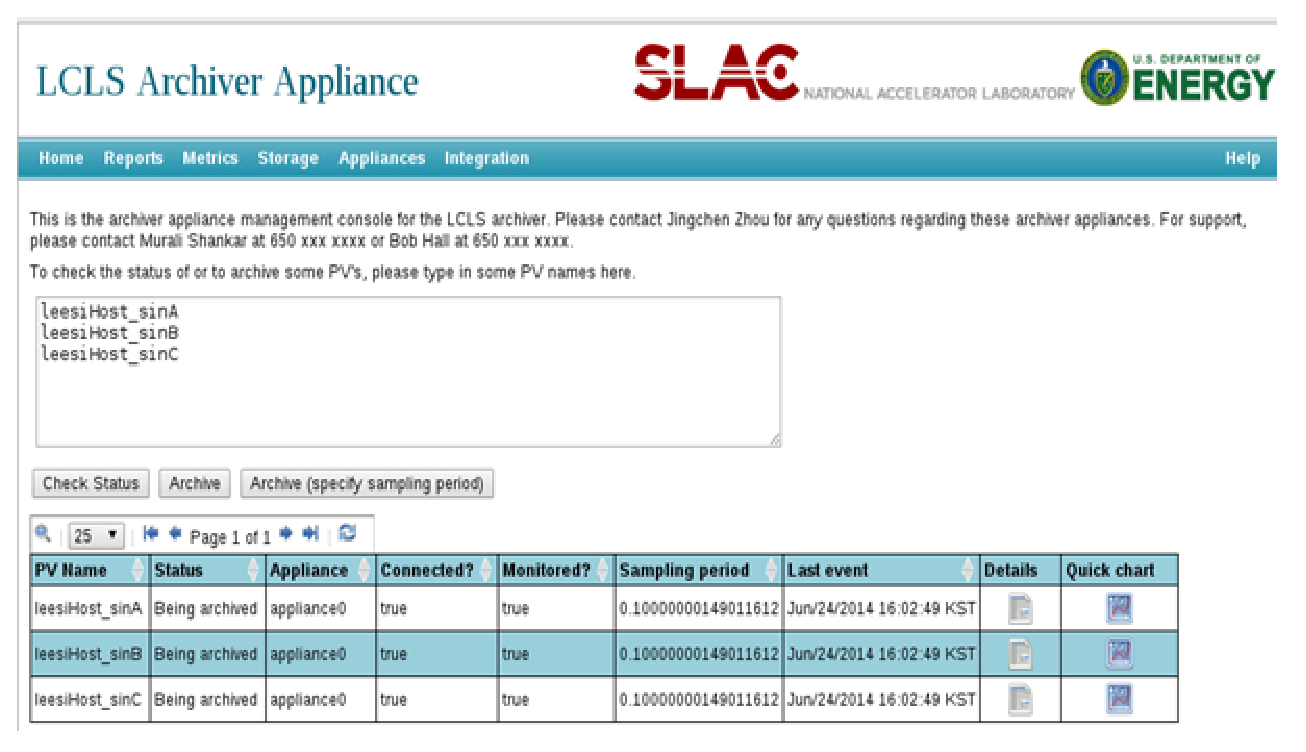
\includegraphics[width=0.85\textwidth, height=0.5\textwidth]{./images/image-5.eps}
		\caption{Management Archiver Appliance} 
	\end{figure}
\begin{itemize}
	\item Starting Archive\\
	Enter the PV to be stored in the listbox and then click on the ``Archive" button:``Initial sampling" status in a while in the standby mode and starts to store data after changed to "Being archived" status. (STS area)
	\clearpage
	\item Sampling rate changes and save policy change\\
	"Archive (specific sampling period)", click the button: You can change the PV-specific sampling rate, and storage policies.
	Saving policy is defined in policies.py.
		\begin{figure}[h!]
			\centering
			\includegraphics[width=0.5\textwidth, height=0.3\textwidth]{./images/9.png}
			\caption{Specific sampling period for PV}
		\end{figure}
	\item Report menu \\
	Show information about PV information applied to the appliance. Clicking on the ``Details" button, you can set the detailed information and basic parameters of each PV. In addition, it is possible to stop, restart or a delete the PV. 
	\begin{figure}[h!]
		\centering
		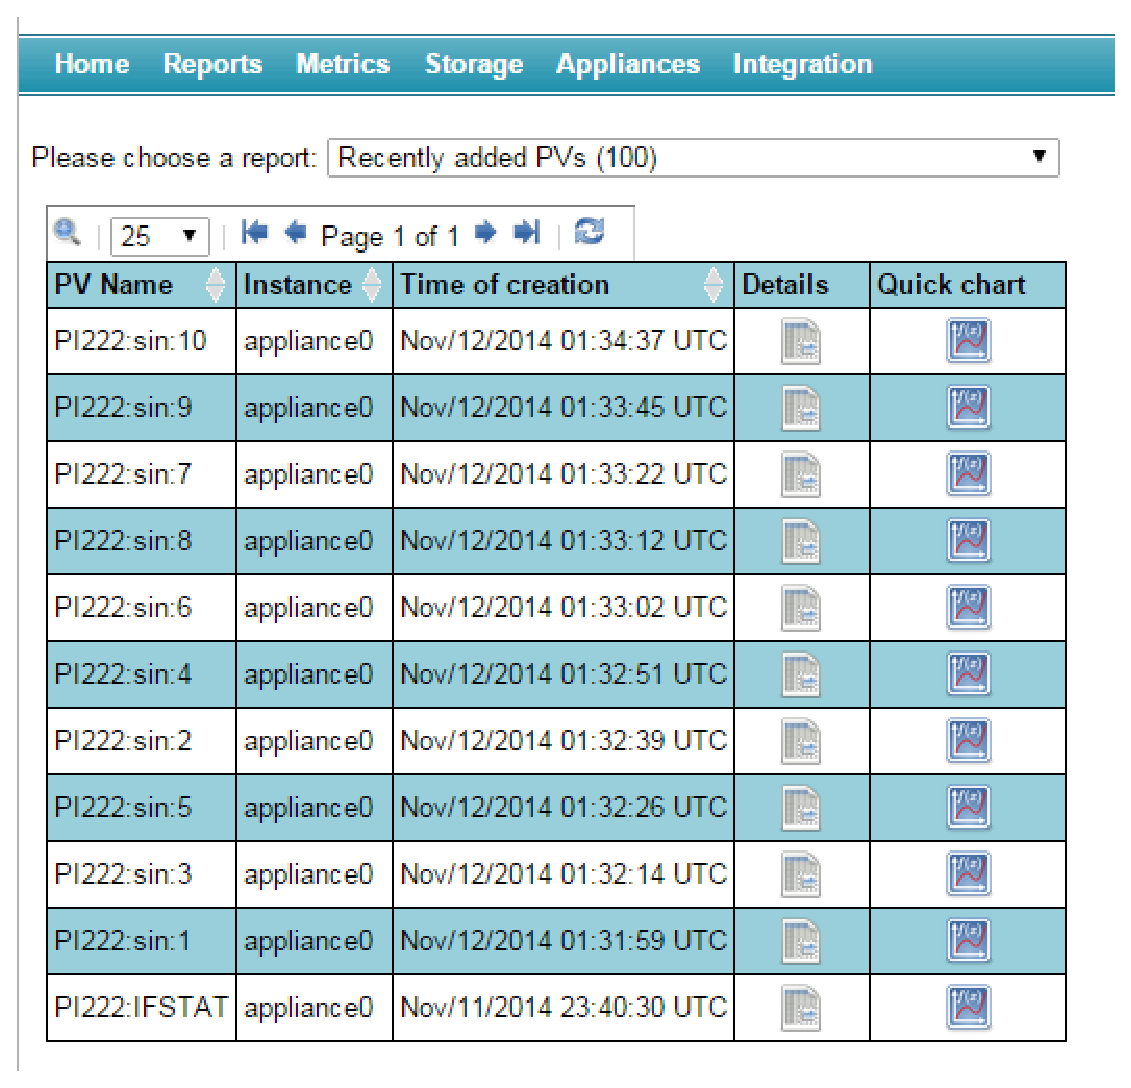
\includegraphics[width=0.85\textwidth, height=0.6\textwidth]{./images/report.eps}
		\caption{Report menu}
	\end{figure}
	\clearpage
	
	\item Metrics menu \\
	 shows the properties for each appliance of clustered appliances. Summary of the main contents to appear at the top of the screen. The contents of the bottom means a property value representing the performance parameters for using the resource in the storage area being used by the appliance.
	
	\begin{figure}[h!]
		\centering
		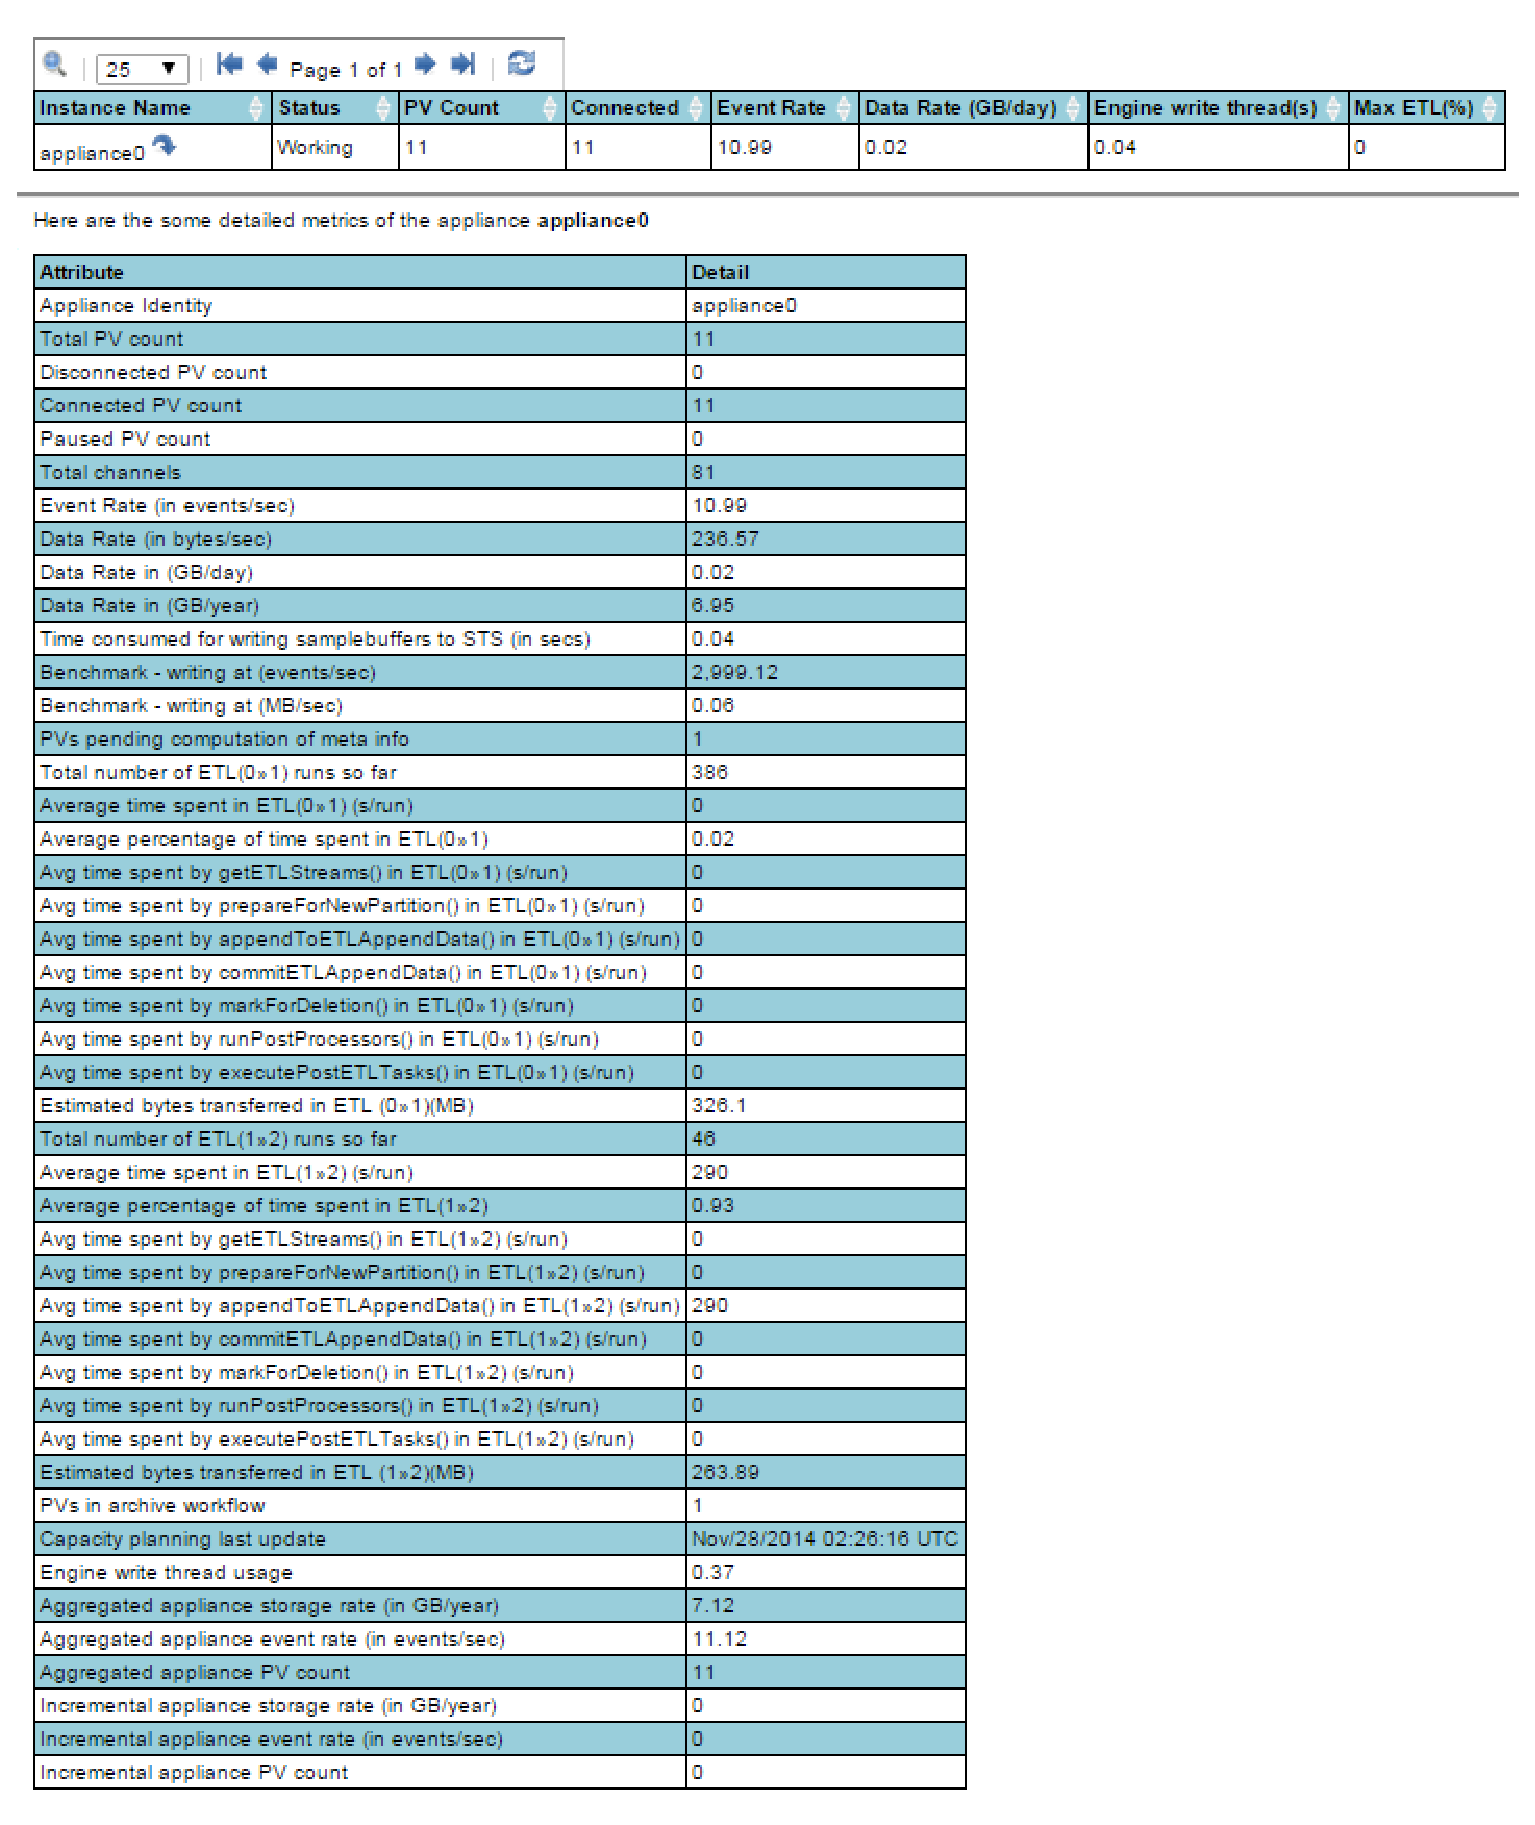
\includegraphics[width=0.85\textwidth, height=0.8\textwidth]{./images/metrics.eps}
		\caption{Metrics menu}

	\end{figure}
	\clearpage
	
	\item Storage menu \\
	The main information about the resources being used in the storage of the appliance three regions (STS, MTS, LTS).
	
	\begin{figure}[h!]
		\centering
		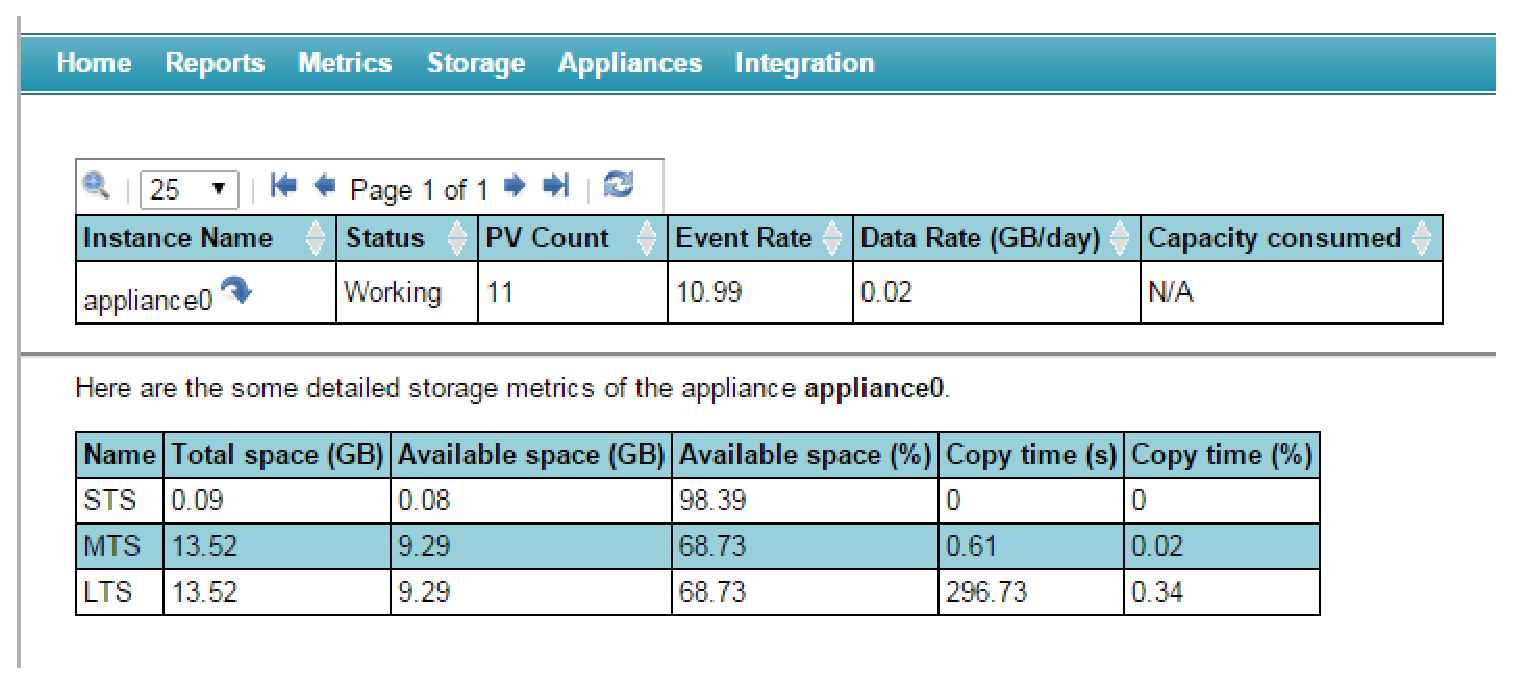
\includegraphics[width=0.85\textwidth, height=0.3\textwidth]{./images/storage.eps}
		\caption{Storage menu}
	\end{figure}
	
	\item Appliances menu \\
It shows the heap memory usage for MGMT three main modules except the module (Engine, Retrieval, ETL). 
	\begin{figure}[h!]
		\centering
		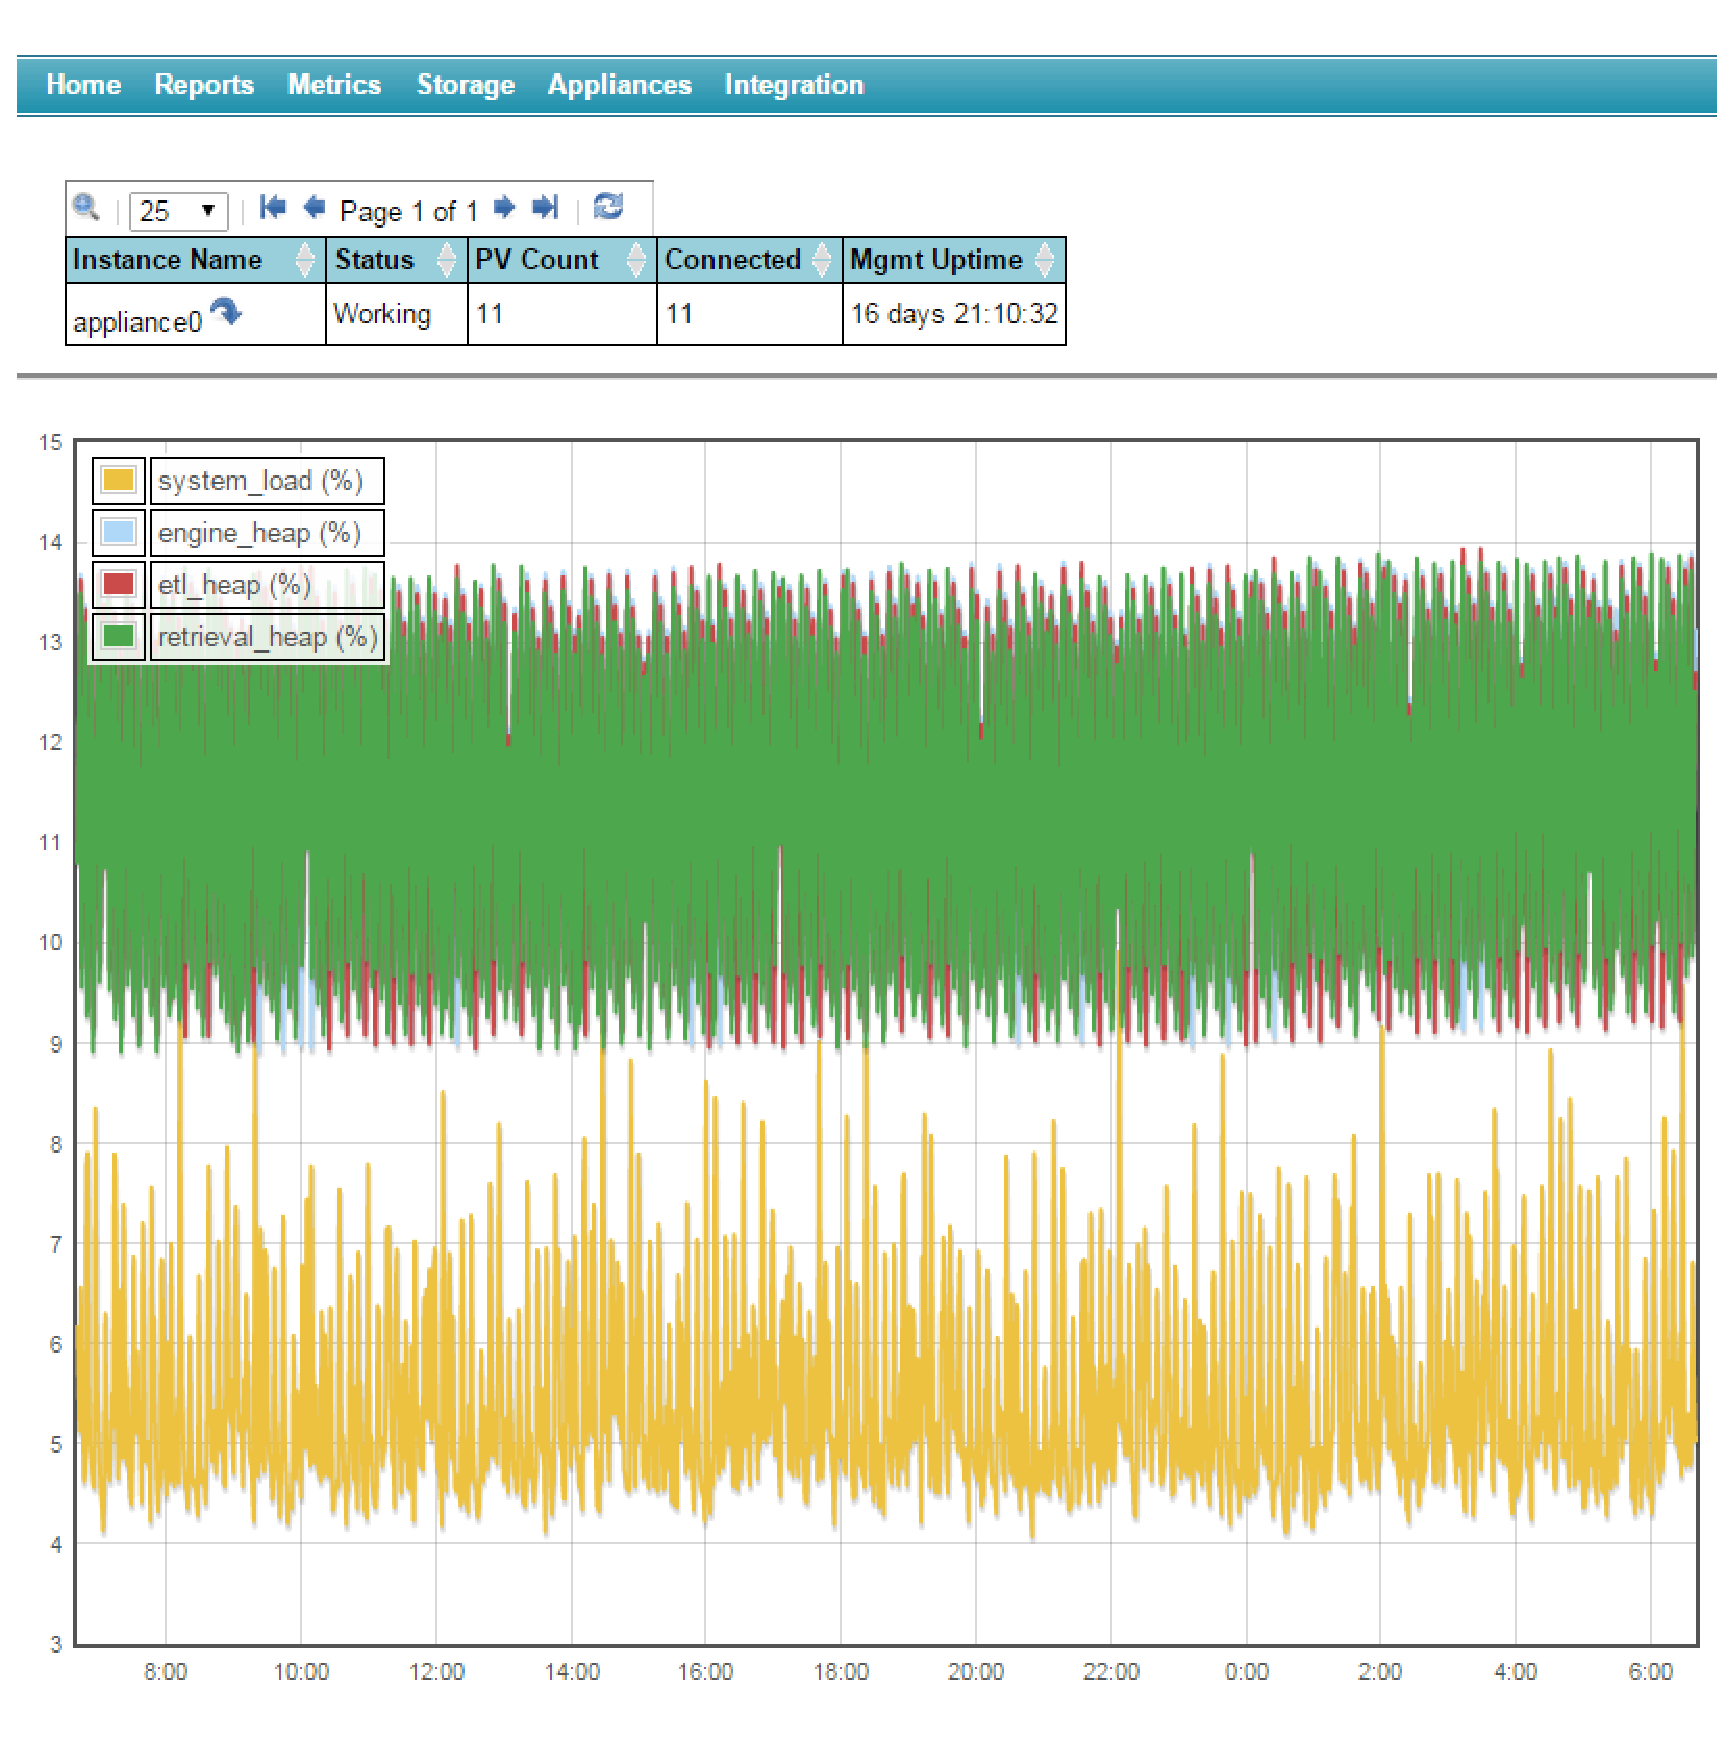
\includegraphics[width=0.85\textwidth, height=0.45\textwidth]{./images/appliance.eps}
		\caption{Appliances menu}
	\end{figure}
	\clearpage
	\item Integration menu \\
	Load a configuration file or a set menu of classic channel archiver to extract the data.
	\begin{figure}[h!]
		\centering
		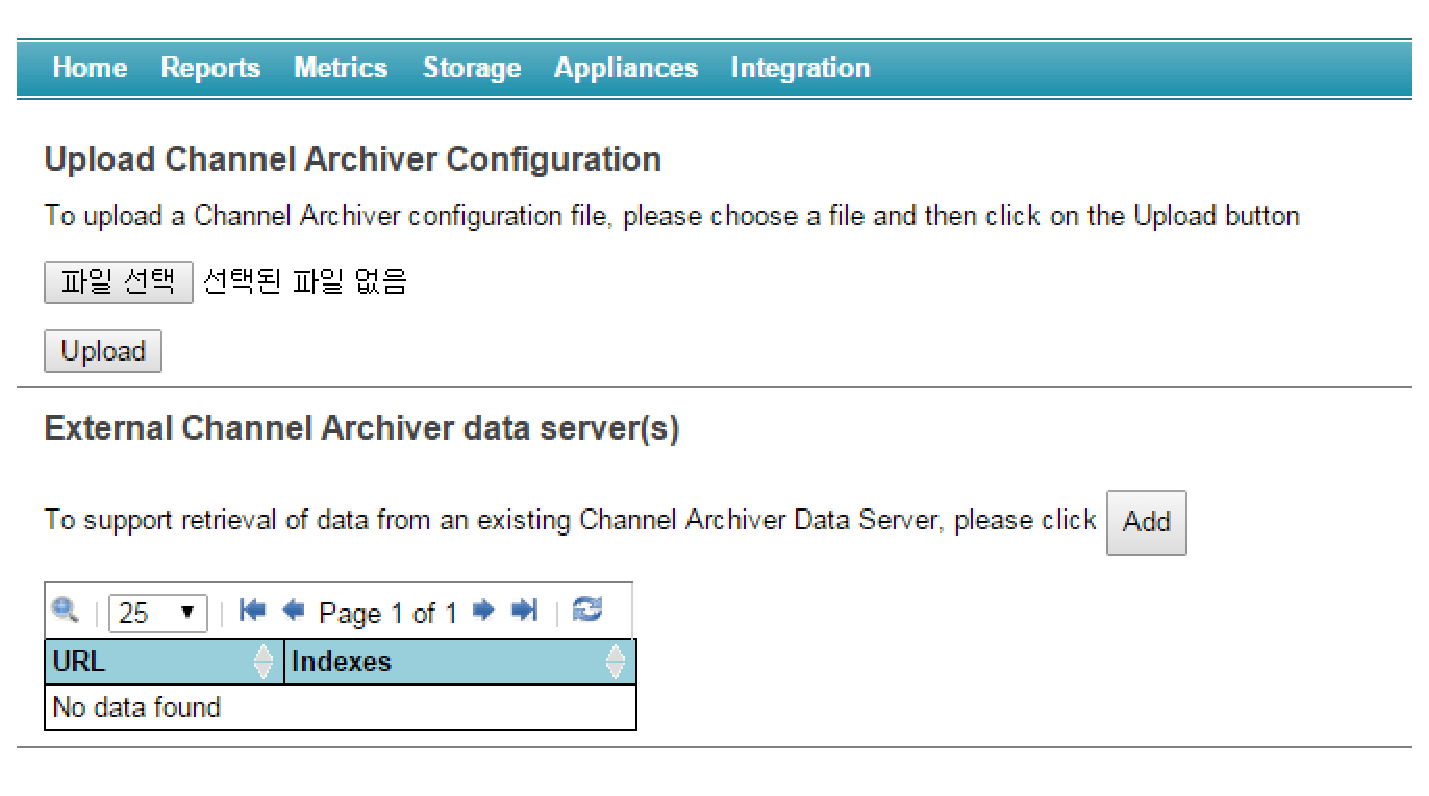
\includegraphics[width=0.85\textwidth, height=0.3\textheight]{./images/integration.eps}
		\caption{Integration menu}
	\end{figure}
\end{itemize}

\clearpage
\chapter{RAON Signal Archiving System}

안정된 가속기 운전을 위해서 중이온가속기구축 사업단의 제어시스템은 실시간 분산 제어 시스템인 EPICS\((Experimental Physics and Industrial Control System\))을 software framework로 사용하고 제어 시스템을 구성하는 모든 장비와 장치에서 나오는 신호 저장 및 관리 역시 EPICS framework을 이용해야하며 각 시설에 맞는 최적화된 신호저장 시스템이 필요하다. EPICS를 framework로 사용하는 신호 저장은 크게 3가지 방법이 있으며 각각의 방법에 따라 동작 방식이 다르다. 본 문서에서는 서로 다른 신호저장 방식에 대한 간략한 설명과 RISP 제어그룹에서 선택한 archiver appliance 유틸리티에 대한 구성 테스트 및 성능 테스트를 통하여 RAON에 맞게 customizing된 신호 저장 시스템의 설계 및 상황에 따른 디자인 방법에 대해서 기술한다.
\section{EPICS Signal Archiver}
EPICS framework를 사용하는 신호 저장은 크게 3가지 방법이 있다. file-base의 접근 방식을 가지는 classic channel archiver, 관계형 데이터베이스를 사용하는 RDB channel archiver 그리고 앞의 두 신호 저장 방식의 문제점을 해결한 archiver appliance가 있다. Archiver appliance는 SLAC에서 개발했고 점차적으로 EPICS community에서 사용량이 증가하고 있다.
\subsection{Classic data storing on EPICS}
\begin{itemize}
	\item Classic Channel Archiver\\
	Classic channel archiver는 PV 데이터에 대한 데이터 블럭의 정보를 담고있는 index file이 존재하며 해당 index 파일의 정보를 통해 데이터 블럭에 접근하여 데이터를 획득한다. 저장을 위한 PV list가 많거나 sampling rate가 높은 PV를 오랜시간 저장해 index file의 크기가 2Gbyte를 넘을 경우 index file을 관리하는 모듈에 성능 부하가 발생하여 데이터 저장 성능이 급속히 떨어진다. 또한 시스템의 임의적인 재부팅 또는 archiver engine의 이상으로 engine을 강제 종료시 특정 데이터 블럭과 index file간의 불일치가 발생하며 이 경우 해당 데이터 블럭을 읽을 수 없는 문제점이 있다.
	\begin{itemize}
		\item 문제점
		\begin{itemize}
			\item Index file size
			\item Index와 data block 간의 불일치
		\end{itemize}
		\item 성능
		\begin{itemize}
			\item 60000 sample/sec
		\end{itemize}
	\end{itemize}
	\item RDB Channel Archiver\\
	Relational DataBase를 사용하는 RDB archiver는 기존 classic channel archiver에서 가지는 index file의 제약 사항에서 벗어 났으며, 범용적으로 사용되는 SQL 쿼리 문을 통해 사용자가 데이터를 자유롭게 추출 할 수 있어 client 프로그램 개발에 많은 자유도를 부여 할 수 있게 되었다. 하지만 내부 동작 매커니즘이 까다로우며 결과적으로 file I/O 성능 상에 문제점이 있다.
	\begin{itemize}
		\item 문제점
		\begin{itemize}
			\item Low performance
			\item 중앙 집중식 데이터 분산 처리의 어려움
		\end{itemize}
		\item 성능
		\begin{itemize}
			\item 7000 sample/sec
		\end{itemize}	
	\end{itemize}
\end{itemize}
\subsection{New approach for storing of EPICS data}
\begin{itemize}
	\item Archiver Appliance
	\begin{itemize}
		\item classic channel archiver와 RDB channel archiver의 문제점을 해결한 유틸리티
	\end{itemize}
\end{itemize}
\section{Signal Archiving System Configuration}
Archiver appliance는 classic channel archiver에서 문제되고 있는 index 파일을 가지는 구조를 제거하였으며, file I/O 성능을 극대화하기 위한 방식으로 로컬파일시스템과 메모리 맵핑되는 RAM filesystem을 사용하였다. 또한 Single Archiver Appliance를 그대로 확장하여 Multiple Archiver Appliance를 구성하여 기존에 문제가 되었던 확장성을 해결하였으며 이러한 확장성은 데이터 저장 시스템을 클러스터 형태로 설게가 가능하도록 하였으며, 데이터 추출도 병렬로 처리하여 부하분산과 데이터 추출 속도를 혁신적으로 단축 시켰다.
\subsection{Archiver appliance를 이용한 신호 저장 시스템 구축}
\begin{itemize}
	\item 계층적 스토리지 영역에 대한 설계
	\item LTS 시스템에 대한 설계 및 정책 디자인
	\item Mutiple archiver appliance의 구현
	\item Apache load balancer를 통한 대량의 데이터 획득에 대한 성능 검증
\end{itemize}
\subsection{계층적 스토리지 영역에 대한 설계 및 LTS 설계}
Archiver appliance의 저장영역은 STS(Short Term Storage)=RAM disk(ramfs), \\MTS(Medium Term Storage)=SAS(ext4), 및 LTS(Long Term Storage)=Network(SAN)로 구성된다. STS영역은 appliance가 기동되면서 가용할 수 있는 메모리의 범주를 확인하여 메모리 영역과 파일 시스템 영역을 맵핑하는 RAM disk의 ram file system을 사용한다. 이는 로컬 영역에서 파일 I/O 성능을 극대화하는 방법으로 사용된다. MTS 영역은 일반적인 SAS disk로 구성되며 multiple archiver appliance의 구성시 appliance의 node down이 발생했을때 down된 노드의 data를 retrieval 시키기 위해서는 각 appliance의 MTS를 네트워크 스토리지로 옮겨야 한다. LTS 영역은 일반 ethernet 네트워크를 통하여 구성할 수 있으며 SAN(Storage Area Network)를 이용하여 구성했다. SAN Storage는 서버 다운없이 대규모 확장이 가능하며 파이버 채널을 이용 기존의 네트워크 스토리지(NAS:Network Attached Storage)의 패킷 사이즈 제한으로 인한 성능제약을 해결 했으며 저장 데이터의 안전과 신속한 복구가 가능하다.

	\begin{figure}[h!]
		\centering
		\includegraphics[width=0.85\textwidth, height=0.3\textheight]{./images/878.png}
		\caption{계층적 스토리지 영역 설계}
	\end{figure}

\subsection{Multiple achiver appliance 구성}
Multiple archiver appliance는 여러개의 single node archiver appliance를 클러스터링을 통해 사용한다. 클러스터의 각 node들은 독립적이지만 load balancing을 통해 제어 할수 있다. load balancin은 하나의 서비스가 발생하는 트래픽이 많을시 여려 대의 서버가 트래픽을 분산처리하여 서버의 로드율 증가, 부하량, 속도저하등을 고려하여 적절히 분산처리해주는 서비스이다. 본 문서의 multiple archiver appliance는 2개의 single node archiver appliance를 이용하였으며, 갂각의 single node archiver appliance는 독립적으로 작동하고 apache load balancing을 이용하여 통합적으로 제어 가능하다. Multiple archiver appliance의 노드는 appliances.xml 파일 수정을 통해 필요한만큼 확장할 수 있다. 이를 통해 데이터 저장 환경에 따라 시스템을 디자인 할 수 있으며 이를 위해서 single node archiver appliance 성능 테스트가 필요하다.

	\begin{figure}[h!]
		\centering
		\includegraphics[width=0.85\textwidth, height=0.4\textwidth]{./images/123.png}
		\caption{Apache load balancing}
	\end{figure}

	\begin{figure}[h!]
		\centering
		\includegraphics[width=0.85\textwidth, height=0.6\textwidth]{./images/789456.png}
		\caption{Multiple archiver appliance homepage}
	\end{figure}


Multiple archiver appliance의 사용은 single node archiver appliance와 같으며 각각의 노드에 접속할 필요없이 각 노드들을 apache mulitple archiver appliance 홈페이지에서 통합적으로 제어 할 수 있다. 저장할 PV를 입력하면 load balancing을 통해 PV를 각 노드로 자동으로 나누어 할당하며 데이터 추출도 load balancing을 사용하여 이루어진다.
\clearpage
\subsection{Hardware 구성}
계층적 스토리지 영역에 대한 설계를 바탕으로 하드웨어 구성을 완료하였다. 
	\begin{figure}[h!]
		\centering
		\includegraphics[width=1\textwidth, height=0.7\textheight]{./images/124.png}
		\caption{Signal Archiving System 랙 구성}
	\end{figure}
\clearpage
	\begin{figure}[h!]
		\centering
		\includegraphics[width=0.85\textwidth, height=0.5\textheight]{./images/125.png}
		\caption{Signal Archiving System 구성}
	\end{figure}
	네트워크 스토리지는 LTS영역에 GPFS와 Lustre를 사용 할 수 있도록 구성했고, 이를 통해 하드웨어의 구성이 이루어 졌다. SAN storage와의 통신을 위해서 SAN switch를 사용하고, SAN switch는 바로 상위단의 서버 2개와 병렬로 연결 되었다. 이 2개의 서버는 GPFS를 LTS로 사용하는 archiver appliance node역할과 Lustre를 위한 OSS 역할을 동시에 수행한다. 이 서버 상위단에는 Lustre를 LTS로 사용하는 multiple archiver appliance를 위한 Lustre client 서버 2개, Lustre client와 Lustre OSS의 연결 및 상위 제어 네트워크 연결을 위한 1Gbps 네트워크 스위치를 사용해서 하드웨어를 구성했다.
	
	\clearpage
	
	\section{Single Node Archiver Appliance 테스트}
	Single node archiver appliance 테스트를 통해 multiple archiver appliance를 구성하기 위한 기본 자료를 획득할 수 있으며, EPICS community에서 이루어 지지않은 max sampling rate 측정 등의 community에 공헌 할 수 있는 방향으로 테스트가 이루어 졌다. 테스트는 archiver appliance의 2가지 모드인 Scan Mode와 Monitor Mode 모드 각각에 대해서 테스트 하였다. Scan Mode와 Monitor Mode는 camonitor를 사용하고 유사한 개념을 가지고 있지만 작은 부분이 차이가 있다. Monitor 모드는 sampling period를 이용하여 버퍼의 용량을 계산 후 사용하고 Scan 모드는 엔진 모듈에서 IOC가 보낸 변수를 슬롯에 할당하며 스레드는 슬롯/변수의 값마다 sampling period를 설정하고 저장한다. 아래는 Monitor 모드의 버퍼 용량을 계산하는 방법이다.
	
	\begin{lstlisting}[style=termstyle]
	int buffer_capacity = ((int) Math.round(Math.max((write_period/pvSamplingPeriod)*sampleBufferCapacityAdjustment, 1.0))) + 1;
\end{lstlisting}
	\subsection{Test 환경}
	\begin{itemize}
		\item Intel(R) Xeon(R) CPU E5-2650 v2 2.6GHz(16-cores)
		\item STS : tmpfs\\
		MTS : SAS\\
		LTS : GPFS
	\end{itemize}
	
	Single node archiver appliance는 GPFS 상위단의 node1에 설치 후 동작 시켰고, CPU time 사용 간섭을 최소화 시키기 위해서 IOC는 GPFS 상위단의의node2에서 동작 시켰다. single node file I/O 성능시험은 제어그룹의 archiver appliance 구성 technical document에 나와있으며 본 문서에서는 언급은 생략한다.
	
	\subsection{testIOC 생성}
	Single node archiver appliance 테스트를 위해 testIOC를 생성하였으며 많은 PV에 따른 IOC의 부담을 최소화 시키기 위해서 10Hz로 작동하는 5000개의 PV를 가지는 IOC 9개 생성하였다. Multiple IOC에서 생성되는 PV 데이터는 sin wave 형태의 data이며 10Hz로 동작한다. testIOC를 만드는 과정은 다음과 같다.
	\begin{itemize}
		\item IOC 디렉토리 생성
		\begin{lstlisting}[style=termstyle]
		[root@root]# mkdir testIOC
		[root@root]# cd testIOC
		\end{lstlisting}
		\item application 생성
		\begin{lstlisting}[style=termstyle]
		[root@root testIOC]# makeBaseApp.pl -t ioc testIOC
		\end{lstlisting}
		\item iocboot 생성
		\begin{lstlisting}[style=termstyle]
		[root@root testIOC]# makeBaseApp.pl -i testIOC
		\end{lstlisting}
		\item Db 생성 (test1.vdb)
		\begin{lstlisting}[style=termstyle]
		record(calc, "$(user):phase:$(NUM)") 
		{
		field(SCAN, ".1 second")
		field(FLNK, "$(user):fanout:$(NUM)")
		field(CALC, "(A>3.141592*2)?0:A+0.01")
		field(INPA, "$(user):phase:$(NUM)")
		field(PREC, "4")
		}
		
		record(calc, "$(user):sinA:$(NUM)")
		{
		field(CALC, "sin(A)")
		field(INPA, "$(user):phase:$(NUM)")
		}
		
		
		record(fanout, "$(user):fanout:$(NUM)")
		{
		field(LNK1, "$(user):sinA:$(NUM)")
		}
		\end{lstlisting}
		\begin{lstlisting}[style=termstyle]
		[root@node2 Db]# ls
		Makefile  O.linux-x86_64  test2.vdb  test4.vdb  test6.vdb  test8.vdb
		O.Common  test1.vdb       test3.vdb  test5.vdb  test7.vdb  test9.vdb
		\end{lstlisting}
		\item Makefile 수정
		\begin{lstlisting}[style=termstyle]
		TOP=../..
		include $(TOP)/configure/CONFIG
		#----------------------------------------
		#  ADD MACRO DEFINITIONS AFTER THIS LINE
		
		#----------------------------------------------------
		#  Optimization of db files using dbst (DEFAULT: NO)
		#DB_OPT = YES
		
		#----------------------------------------------------
		# Create and install (or just install) into <top>/db
		# databases, templates, substitutions like this
		#DB += xxx.db
		DB += test1.vdb
		DB += test2.vdb
		DB += test3.vdb
		DB += test4.vdb
		DB += test5.vdb
		DB += test6.vdb
		DB += test7.vdb
		DB += test8.vdb
		DB += test9.vdb
		#----------------------------------------------------
		# If <anyname>.db template is not named <anyname>*.template add
		# <anyname>_template = <templatename>
		
		include $(TOP)/configure/RULES
		#----------------------------------------
		#  ADD RULES AFTER THIS LINE
		\end{lstlisting}
		\item src 생성\\
		synApp의 seq 모듈의 example을 이용하여 src를 생성해준다.
		\item st.cmd 생성 (st1.cmd)
		\begin{lstlisting}[style=termstyle]
		#!../../bin/linux-x86_64/testIOC
		
		## You may have to change testIOC to something else
		## everywhere it appears in this file
		
		< envPaths
		
		cd "${TOP}"
		
		## Register all support components
		dbLoadDatabase "dbd/testIOC.dbd"
		testIOC_registerRecordDeviceDriver pdbbase
		
		## Load record instances
		#dbLoadTemplate "db/userHost.substitutions"
		#dbLoadRecords "db/dbSubExample.db", "user=rootHost"
		dbLoadRecords("db/test1.vdb","user=namsh, NUM=000001")
		dbLoadRecords("db/test1.vdb","user=namsh, NUM=000002")
		dbLoadRecords("db/test1.vdb","user=namsh, NUM=000003")
		dbLoadRecords("db/test1.vdb","user=namsh, NUM=000004")
		dbLoadRecords("db/test1.vdb","user=namsh, NUM=000005")
		.
		.
		.
		.
		.
		dbLoadRecords("db/test1.vdb","user=namsh, NUM=004996")
		dbLoadRecords("db/test1.vdb","user=namsh, NUM=004997")
		dbLoadRecords("db/test1.vdb","user=namsh, NUM=004998")
		dbLoadRecords("db/test1.vdb","user=namsh, NUM=004999")
		dbLoadRecords("db/test1.vdb","user=namsh, NUM=005000")
		
		## Set this to see messages from mySub
		#var mySubDebug 1
		
		## Run this to trace the stages of iocInit
		#traceIocInit
		
		cd "${TOP}/iocBoot/${IOC}"
		iocInit
		
		## Start any sequence programs
		#seq sncExample, "user=rootHost"
		\end{lstlisting}
		\begin{lstlisting}[style=termstyle]
		[root@node2 ioctestIOC]# ls
		envPaths  README   st2.cmd  st4.cmd  st6.cmd  st8.cmd
		Makefile  st1.cmd  st3.cmd  st5.cmd  st7.cmd  st9.cmd
		\end{lstlisting}
		
	\end{itemize}

	\subsection{Scan Mode 테스트}
	Scan 모드는 엔진 모듈에서 IOC가 보낸 변수를 슬롯에 할당하며 스레드는 슬롯/변수의 값마다 sampling period를 설정하고 저장한다. 테스트는 10Hz로 동작하는 45000개의 PV를 아카이빙 했다. Archive는 스캔 모드, sampling period는 0.1 sec, 정책은 default(STS : 1시간, MTS : 1일, LTS : 1년)를 선택했고, 45000개의 PV는 archive 즉시 inital sampling을 시작했다. PV는 archive workflow에 대기 후 engine write에 따라서 1000개씩 순서대로 count 되고, 1개의 PV count 마다 8개의 채널이 생성 되었다.  
	\begin{figure}[h!]
			\centering
			\includegraphics[width=1\textwidth, height=0.25\textheight]{./images/channel.png}
			\caption{PV수에 따른 channel수 변화}
	\end{figure}
		
	Scan 모드 테스트에서 시간에 따른 PV 변화는 PV수가 늘어남에 따라서 workflow에서 PV가 count되는데 걸리는 시간이 점점 늘어남을 확인할 수 있다.
	\begin{figure}[h!]
		\centering
		\includegraphics[width=1\textwidth, height=0.25\textheight]{./images/time.png}
		\caption{시간에 따른 PV수 변화}
	\end{figure}
	
	이는  engine thread의 영향으로 PV수가 많아짐에 따라서 엔진 모듈에서 처리해야되는 PV수가 많아져 write thread가 높아져서 발생하는 현상이다. 이것은 Scan 모드의 단점으로 볼 수 있으며 특히 PV수가 36000에서 37000으로 넘어가는 구간은 약 1시간(54분 24초)이 소요되므로 대량의 PV를 저장하는 정책으로는 적합하지 않은 것을 확인할 수 있다. 
	\clearpage
	\begin{figure}[h!]
		\centering
		\includegraphics[width=1\textwidth, height=0.25\textheight]{./images/thread.png}
		\caption{PV수에 따른 engine write thread (s) 변화}
	\end{figure}

PV수에 따라서 쌓이는 data는 점점 늘어 났으며 PV수에 따라서 데이터가 일정하게 늘어나지 않는 것으로 보아 버퍼의 영향으로 data loss가 생기는 것을 확인 할 수 있다. Data rate는 PV 수가 36000일때 3767794.09 byte/sec(3.5932 MB/sec), 303.18 GB/day, 110660.82 GB/year으로 가장 높았고, 이후 점점 하락해 PV 수가 37000일때 3652455.06 byte/sec(3.4832 MB/sec), 293.9 GB/day, 107273.29 GB/year로 나타났다. Scan mode를 사용할때에 appliance에서 받는 데이터는 최대 3.5932 MB/sec로 어플라이언스와 상위 네트워크 간의 연결은 1Gbps(125 MB/sec)를 사용하여도 충분함을 확인 할 수 있고, 1년동안 저장되는 data 양이 최대 108 TB/year로 LTS 서버의 확장성에 따라 data를 저장하는데 충분히 문제가 없음을 확인했다. 하지만 data loss가 생기는것을 확인 하였음으로 data loss가 일어 나지 않는 archiver appliance 정책 및 시스템 디자인이 필요하다.
	
	\begin{figure}[h!]
		\centering
		\includegraphics[width=1\textwidth, height=0.3\textheight]{./images/sec.png}
		\caption{PV수에 따른 data rate (byte/sec) 변화}
	\end{figure}
	\clearpage
	\begin{figure}[h!]
		\centering
		\includegraphics[width=1\textwidth, height=0.25\textheight]{./images/day.png}
		\caption{PV수에 따른 data rate (GB/day) 변화}
	\end{figure}
	\begin{figure}[h!]
		\centering
		\includegraphics[width=1\textwidth, height=0.25\textheight]{./images/year.png}
		\caption{PV수에 따른 data rate (GB/year) 변화}
	\end{figure}


	Sampling rate는 data rate와 비슷한 추세로 36000개의 PV가 connection 되었을때 190145.12로 가장 높았고 이후 184000(184579.58)대로 하락하여 37000개의 PV가 connection 되었을때도 184000대의 sampling rate를 유지하였다. Scan 모드로 동작하는 single mode archiver appliance의 최대 samping rate는 약 190000으로 확인 할 수 있었으며, 10Hz로 동작하는 37000개의 PV를 아카이빙 하였음으로 370000Hz의 sampling rate를 가져야 하지만 190000의 sampling rate를 가지므로 약 180000의 data loss가 발생한 것을 확인했다.
	\clearpage
		\begin{figure}[h!]
			\centering
			\includegraphics[width=1\textwidth, height=0.25\textheight]{./images/samplingrate.png}
			\caption{PV수에 따른 sampling rate 변화}
		\end{figure}

신호 저장 시스템의 신뢰성과 안정성을 위해서 single node archiver appliance에서 data loss가 발생하지않는 smapling rate를 찾기위해 sampling rate를 낮춰가며 확인했다. 10Hz sampling period로 1000개의 PV를 입력하여 10000Hz에서 data loss가 발생하는 것을 확인 했으며, 각 PV 마다 10초에 1개에서 2개의 data loss가 일어났다.
		\begin{figure}[h!]
			\centering
			\includegraphics[width=1\textwidth, height=0.5\textheight]{./images/a1.png}
			\caption{10000Hz(10Hz,1000PV) sampling시 data loss}
		\end{figure}

10초마다 일정한 간격으로 data loss가 일어나는 현상이 있었고, 이 현상이 buffer에의한 문제인지 아니면 archiver appliance의 내부 알고리즘의 문제인지 확인하기 위해서 5Hz의 sampling period로 2000개의 PV를 저장하는 테스트와 1Hz의 sampling period로 10000개의 PV를 저장하는 테스트를 실행했다.

		\begin{figure}[h!]
			\centering
			\includegraphics[width=1\textwidth, height=0.1\textheight]{./images/a3.png}
			\caption{10000Hz(5Hz,2000PV) sampling시 data loss}
		\end{figure}
	
5Hz sampling period로 2000개의 PV를 저장시 10000Hz의 event rate가 나와야 하지만 event rate는 9802.57로 초당 197.43의 data loss가 발생함을 확인했고, 이는 평균적으로 1개의 PV가 초당 약 0.2의 data loss를 가지는것을 의미한다. 이를 통해 1개의 PV에서 10초당 1개에서 2개의 data loss가 발생함을 예측할 수 있다.
		\begin{figure}[h!]
			\centering
			\includegraphics[width=1\textwidth, height=0.5\textheight]{./images/a2.png}
			\caption{10000Hz(5Hz,2000PV) sampling시 data loss}
		\end{figure}

결과적으로 5Hz sampling period로 2000개의 PV를 저장시 10Hz sampling period로 1000개의 PV를 저장 할때와 같은 현상이 일어 났다. 이를 통해 10초 주기로 data loss가 발생하는 이유는 archiver appliance의 내부적인 알고리즘 문제가 아니며, data loss가 발생하는 이유는 buffer의 overflow에 의한 현상임을 확인했다. Buffer의 overflow에 의한 현상은 시스템 메모리의 추가로 개선의 여지가 있으며, 신호 저장 시스템 설계시 시스템 메모리도 설계의 중요사항으로 볼 수 있다.

		\begin{figure}[h!]
			\centering
			\includegraphics[width=1\textwidth, height=0.5\textheight]{./images/a4.png}
			\caption{10000Hz(1Hz,10000PV) sampling시 data loss}
		\end{figure}
		
\subsection{Monitor Mode 테스트}
Monitor 모드는 설정한 sampling period를 이용하여 버퍼의 용량을 미리 계산한뒤 사용하는 방식으로 scan 모드와는 조금의 차이점이 있다. 테스트는 scan 모드와의 차이점을 보기 위해서 scan 모드와 동일하게 진행 되었다. Archive는 Monitor 모드, sampling period는 0.1 sec, 정책은 default(STS : 1시간, MTS : 1일, LTS : 1년)를 선택했고, 45000개의 PV는 archive 즉시 inital sampling을 시작했다. PV는 archive workflow에 대기 후 engine write에 따라서 1000개씩 순서대로 count되고, 1개의 PV count 마다 8개의 채널이 생성되었다.
\clearpage

		\begin{figure}[h!]
			\centering
			\includegraphics[width=1\textwidth, height=0.3\textheight]{./images/channel1.png}
			\caption{PV 수에 따른 channel 수 변화}
		\end{figure}

Monitor 모드 테스트에서 시간에 따른 PV 변화는 PV 수가 늘어남에도 workflow에서 PV가 count 되는데 걸리는 시간은 약 2분 정도로 거의 일정 하였으며 engine write thread의 변화는 scan 모드와 비슷하지만 count되는 시간이 거의 일정한 이유는 engine thread에 상관없이 monitor 모드에서는 버퍼의 용량을 미리 계산하고 사용하기 때문으로 보인다.

		\begin{figure}[h!]
			\centering
			\includegraphics[width=1\textwidth, height=0.3\textheight]{./images/pv1.png}
			\caption{PV 수에 따른 channel 수 변화}
		\end{figure}
\clearpage
\begin{figure}[h!]
	\centering
	\includegraphics[width=1\textwidth, height=0.3\textheight]{./images/thread1.png}
	\caption{PV 수에 따른 engine write thread (s) 변화}
\end{figure}

Monitor 모드는 PV가 늘어남에 따라 데이터가 거의 일정하게 늘어나는것을 확인 할 수 있었으며, 이것은 다량의 PV를 저장하는데 data의 손실률이 적다는 것을 의미한다. Data의 손실률이 적음으로 data rate는 거의 일정하게 증가하였으며, data rate는 PV수가 38000일때 7199415.52 byte/sec(6.8658 MB/sec), 579.31 GB/day, 211448.19 GB/year(206.4923 TB/year)로 가장 높게 나타났고, 38000개 이후의 PV는 서버의 메모리부족으로 확인할 수 없었다. 서버의 메모리를 추가 한다면 이 이상의 event도 저장 가능하다고 판단된다. Monitor 모드 역시 어플라이언스와 상위 네트워크 간의 연결은 1Gbps(125 MB/sec)를 사용하여도 충분함을 확인했고, 1년동안 저장되는 데이터 양이 380000Hz의 event rate가 발생했을때 206 TB정도로 LTS 서버의 확장성을 이용하면 충분히 데이터를 저장할 수있다.

\begin{figure}[h!]
	\centering
	\includegraphics[width=1\textwidth, height=0.3\textheight]{./images/sec1.png}
	\caption{PV 수에 따른 data rate (byte/sec) 변화}
\end{figure}
\clearpage
\begin{figure}[h!]
	\centering
	\includegraphics[width=1\textwidth, height=0.3\textheight]{./images/day1.png}
	\caption{PV 수에 따른 data rate (GB/day) 변화}
\end{figure}
\begin{figure}[h!]
	\centering
	\includegraphics[width=1\textwidth, height=0.3\textheight]{./images/year1.png}
	\caption{PV 수에 따른 data rate (GB/year) 변화}
\end{figure}

Event rate는 data rate와 비슷한 추세로 380000개의 PV가 connection 되었을때 \\363405.53으로 scan 모드에 비해서 월등한 성능을 보였으며 시스템 메모리가 충분하다면 최대 event rate는 이보다 훨씬 더 높을 것으로 보인다. 하지만 40000Hz의 event rate 이후 PV가 추가 될때마다 추가되는 event rate는 점점 하락하는 모습을 보였으며, 이는 data loss의 양이 점점 많아짐을 의미한다. 38000개의 PV를 아카이빙 했을때 380000Hz의 event rate를 가져야 하지만 363495.53의 event rate를 가지므로 초당 16504.47의 data loss가 발생한 것을 확인 했다. 
\clearpage
\begin{figure}[h!]
	\centering
	\includegraphics[width=1\textwidth, height=0.3\textheight]{./images/event1.png}
	\caption{PV 수에 따른 event rate 변화}
\end{figure}
Monitor 모드에서는 buffer overflow에 의한 event drop이 scan모드보다 훨씬 덜 일어나며, 버퍼 용량을 미리 계산하여 사용되므로 시스템 메모리가 충분할때 archiver appliance의 sampling period를 저장하고자하는 PV의 동작 속도보다 높게 설정해 계산되는 버퍼의 용량을 event가 필요로하는 용량 이상으로 잡아서 사용한다면 data loss에 대한 문제를 해결할 수 있을것으로 보인다. 현재 archiver appliance의 최소 sampling period는 0.1, 최대 sampling period는 86400으로 10Hz로 동작하는 IOC의 event보다 높게 설정할 수 없도록 되어있다. 하지만 archiver appliance 홈페이지에서 각 PV의 detail부분을 선택하면 PV의 sampling period를 0.01로도 설정 할 수 있으며, EPICS IOC의 최대 동작이 10Hz이기 때문에 개별적인 sampling period 설정으로 data loss를 막을 수 있다. Data loss를 해결하기위한 다른 방법으로는 FRIB/PSI에서 사용하는 engine의 sample buffer size를 늘이는 방법이다. 기본적으로 적용되어있는 sampleBufferCapacityAdjustment=1로 100\%이지만, sampleBufferCapacityAdjustment=1.5로 변경하면 buffer size를 150\%로 증가시켜 data loss를 막을 수 있다. 하지만 data loss를 줄이기 위한 두 방법 모두 메모리를 사용하기 때문에 대량의 신호를 저장하는 시스템 디자인시 multiple archiver appliance와 사용과 같이 메모리 부분의 디자인도 필요하다.\\
\subsection{결론}
Single node archiver appliance는 scan 모드와 monitor 모드의 테스트로 data loss의 양이 적고 성능적으로 우세한 모드는 monitor 모드로 나타났다. 또한 monitor 모드에서 data loss 부분은 sampling period의 변경과 default buffer size의 변경으로 줄일 수 있어 대량의 데이터를 저장하는데에는 monitor 모드의 사용이 적합하다고 판단된다. 하지만 monitor 모드 역시 시스템 메모리 부족으로 인한 node down이 일어날 수 있으므로 multiple archiver appliance의 사용과 각 노드의 메모리 디자인이 필요하다.


\clearpage
\section{Multiple Archiver Appliance 테스트}
본 문서의 multiple archiver appliance 테스트에서 사용하는 multiple archiver appliance는 2개의 single node archiver appliance를 클러스터링 했다. Multiple archiver appliance의 구성 방법과 사용법 등은 본 문서의 Chapter3 Multiple Archiver Appliance Configuration과 Chater5.2의 Signal Archiving System Configuration 부분을 확인하면 된다.
\subsection{Test 환경}
\begin{itemize}
	\item Archiver Applance Node1\\
	Intel(R) Xeon(R) CPU E5-2650 v2 2.6GHz(16-cores)\\
	STS : tmpfs, MTS : SAS, LTS : SAN(GPFS)
	\item Archiver Appliance Node2\\
	Intel(R) Xeon(R) CPU E5-2620 v2 @ 2.10GHz(12-cores)\\
	STS : tmpfs, MTS : SAS, LTS : SAN(GPFS)
\end{itemize}
\subsection{PV load balancing 확인}
Apache load balancing을 통해 입력된 PV가 각 노드로 나누어져 들어가는지 확인했다.
\begin{figure}[h!]
	\centering
	\includegraphics[width=1\textwidth, height=0.2\textheight]{./images/Selection_007.png}
	\caption{Apache load balancing}
\end{figure}

입력된 PV가 load balancing을 통해 appliance0와 appliance1로 load balancing 되는 것을 확인했다. 각 PV의 데이터는 지정된 노드의 tmpfs에 저장 되었으며 ETL 모듈에 의해 각 노드의 SAS로 저장된 후 네트워크 스토리지인 SAN에 저장되었다.
\subsection{아카이빙중인 PV의 노드변경}
아카이빙중인 PV의 노드변경은 multiple arachiver appliance 홈페이지에서 PV의 Details 부분에서 할 수 있다.
\clearpage
\begin{figure}[h!]
	\centering
	\includegraphics[width=1\textwidth, height=0.2\textheight]{./images/Selection_07.png}
	\caption{아카이빙중인 PV의 노드변경}
\end{figure}

아카이빙중인 PV는 Pause 시키지 않으면 appliance 노드 변경이 불가하므로 노드 변경 전에 Pause 시켜준다. Pause를 하지 않았다면 아래의 그림처럼 통합 할 수 없다는 메세지가 팝업된다.
\begin{figure}[h!]
	\centering
	\includegraphics[width=1\textwidth, height=0.5\textheight]{./images/Selection_006.png}
	\caption{Pause하지 않았을때 발생하는 메세지}
\end{figure}

아카이빙중인 PV의 appliance 노드 변경을 위해서 우측 상단의 Pause archivin을 클릭 후, Change appliance를 클릭하면 노드 변경 창이 팝업된다.
\clearpage
\begin{figure}[h!]
	\centering
	\includegraphics[width=0.8\textwidth, height=0.4\textheight]{./images/Selection_005.png}
	\caption{PV의 details}
\end{figure}
\begin{figure}[h!]
	\centering
	\includegraphics[width=0.8\textwidth, height=0.4\textheight]{./images/Selection_004.png}
	\caption{노드변경 팝업 창}
\end{figure}
Enter the new appliance: 부분에서 변경할 노드를 선택하고 현재까지 저장한 데이터를 어느 곳에 저장 할지 선택한다. 데이터는 STS, MTS, LTS를 선택하여 저장할 수 있다. 데이터 저장은 데이터의 양에 따라 시간이 걸리며, 데이터 저장이 완료된 후에 노드의 변경이 이루어진다. 노드 변경이 완료된 후 Resume archiving을 클릭해서 아카이빙을 재개할 수 있다. 노드변경된 PV는 별도의 initial sampling 과정을 거치지 않으며, 재개와 동시에 아카이빙 된다. 이는 multiple archiver appliance의 특성으로 PV에 대한 정보는 두개의 노드 모두 동일한 MySQL database를 사용하기 때문이다.
\subsection{노드1 mgmt에서 노드2의 정보를 확인하기}
노드1 mgmt에서 확인 가능한 정보는 apache에서 확인 가능한 정보와 같으며, 노드1의 mgmt에서 노드2의 정보 확인, 제어 및 데이터 추출이 가능하다. 하지만 각 노드의 mgmt에서는 apache load balancing을 사용할 수 없으므로 multiple archiver appliance의 사용시에는 apache로 접속하여 정보의 확인 및 제어 하는것을 권장한다.
\\\\
\begin{figure}[!htb]
	\centering
	
	\subbottom[노드1 mgmt Home]
	{
		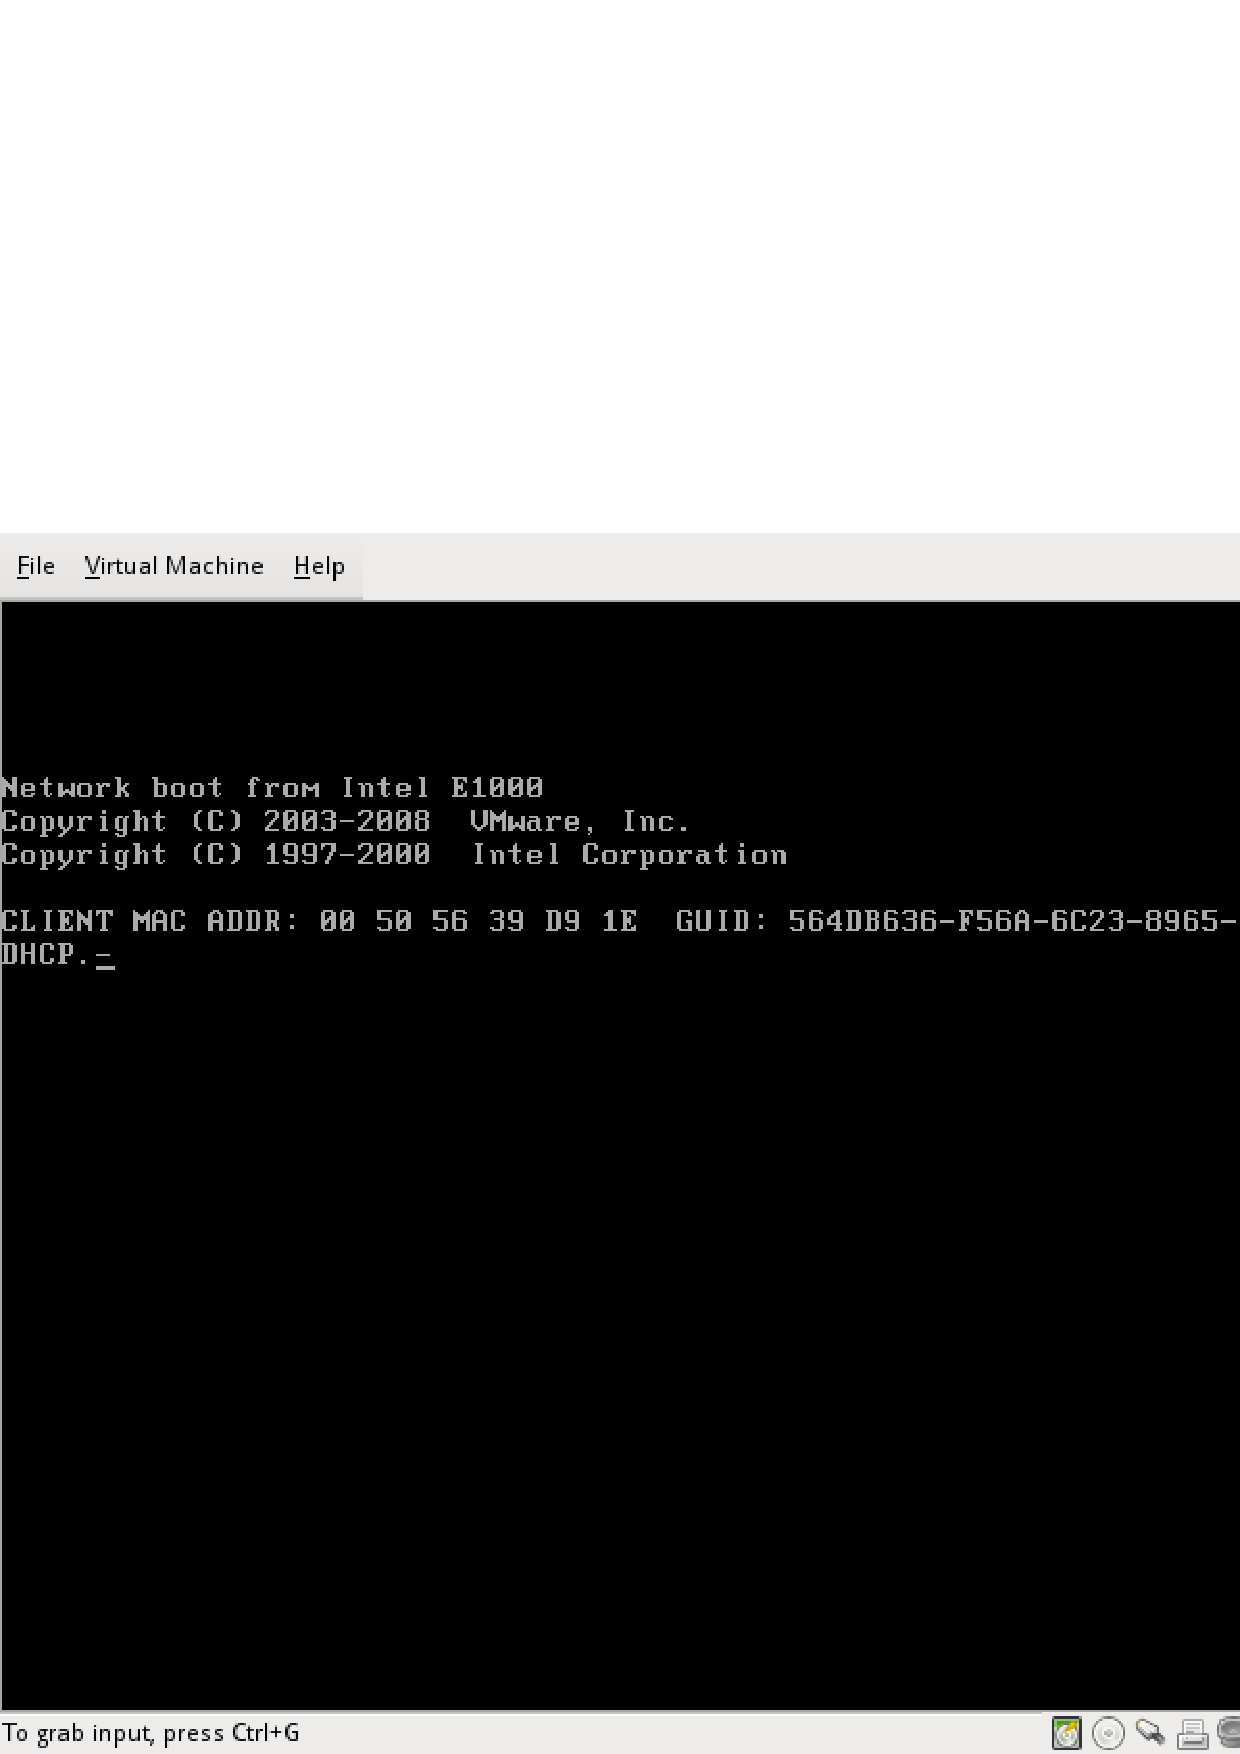
\includegraphics[width=0.45\textwidth]{./images/f-0.png}
		}
	\hfill
	\subbottom[노드1 mgmt Reports]
	{
		\includegraphics[width=0.45\textwidth]{./images/f-1.png}
		}
	\subbottom[노드1 mgmt Metrics]
	{
		\includegraphics[width=0.45\textwidth]{./images/f-2.png}
		}
	\hfill
	\subbottom[노드1 mgmt Appliances]
	{
		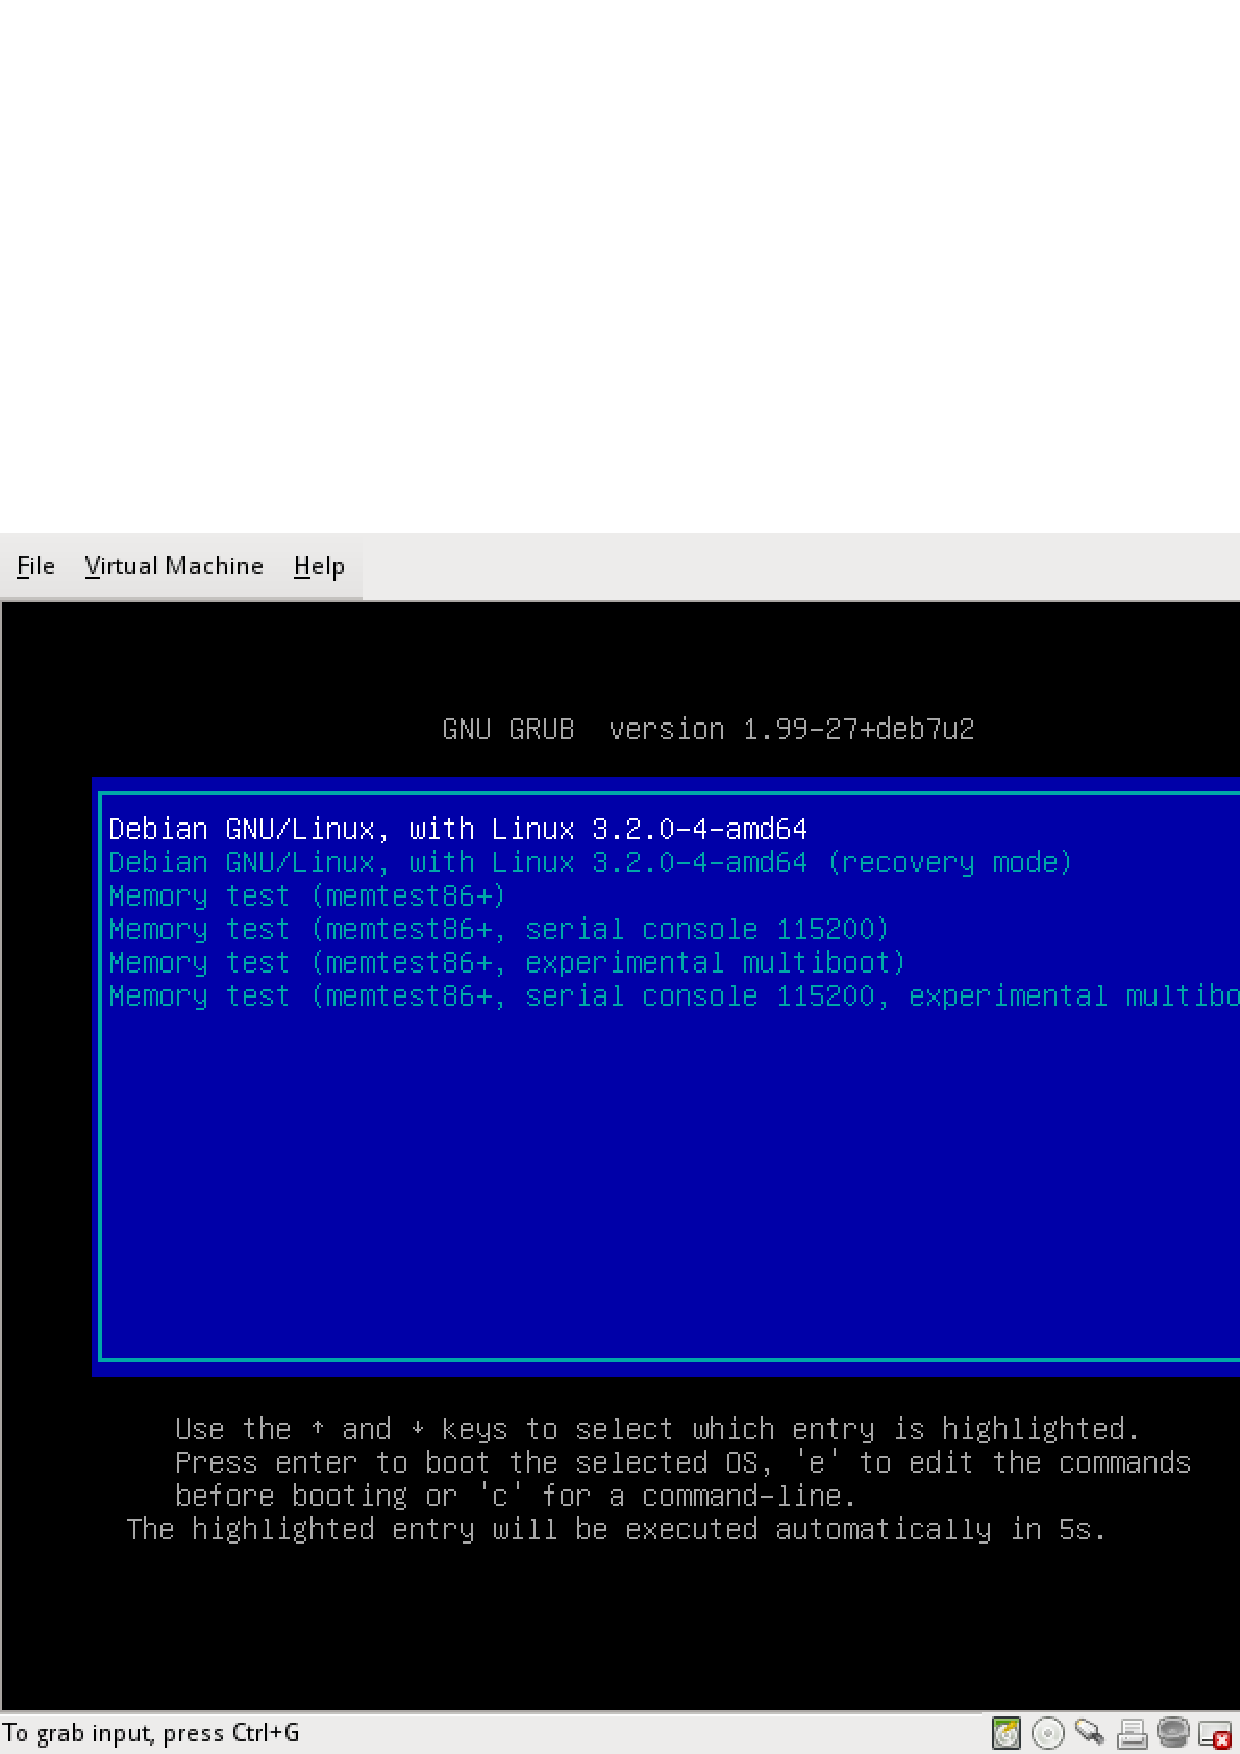
\includegraphics[width=0.45\textwidth, height=0.23\textheight]{./images/f-3.png}
		}
\end{figure}
\clearpage
\subsection{한쪽 노드의 Appliance Down}
Multiple archiver appliance의 동작중 예기치 못한 상황으로 인한 한개의 노드 다운시 mgmt home의 Status 부분에서 Appliance Down 메세지를 확인할 수 있다. Appliance 다운시 mgmt의 모든 메뉴들에서 다운된 노드의 정보는 확인할 수 없다.
\begin{figure}[h!]
	\centering
	\includegraphics[width=0.9\textwidth, height=0.15\textheight]{./images/Selection_012.png}
	\caption{노드2 Appliance Down}
\end{figure}

어느 한쪽 노드가 appliance down 된 상황에서 전체적인 설정을 변경하려고 할때 아래와 같은 메세지가 팝업되며 down되지 않은 노드에는 변경한 설정이 적용된다.
\begin{figure}[h!]
	\centering
	\includegraphics[width=0.85\textwidth, height=0.2\textheight]{./images/Selection_013.png}
	\caption{설정 변경시 에러 메세지}
\end{figure}

다운된 archiver appliance를 재기동시 Status에 Appliance assigned 메세지가 나온다.
\begin{figure}[h!]
	\centering
	\includegraphics[width=0.9\textwidth, height=0.15\textheight]{./images/Selection_014.png}
	\caption{Appliance assigned}
\end{figure}

다운된 archiver appliance의 재기동은 오래 걸리지 않으며, 재기동 된후 다운되기 전의 설정으로 다시 동작한다.
\begin{figure}[h!]
	\centering
	\includegraphics[width=0.9\textwidth, height=0.15\textheight]{./images/Selection_015.png}
	\caption{노드2 활성화}
\end{figure}

노드의 다운된 시간동안 다운된 노드에서 저장중인 PV의 data loss가 발생하며, 활성화중인 노드로 PV의 동적인 재분배는 이루어 지지 않았다. 이를 해결하고 안정적인 사용을 위해 세션 클러스터링을 이용하는 방법이 있다. 세션 클러스터링은 tomcat의 세션이 의도치않게 종료될때 다른 세션이 이를 대체하는 방법이다.\\
한 노드의 appliance down시 다운된 노드 서버에 저장된 데이터는 추출이 불가하며, 다운된 노드의 데이터가 공유되는 네트워크 스토리지에 있다면 추출이 가능하다. 이 때문에 archiver appliance의 MTS도 공유되는 네트워크 스토리지를 사용하는 것이 적절하다.
\clearpage
\section{RISP Archiver Appliance}
Archiver Appliance는 중요한 요소를 건드리지 않는 한도내에서 홈페이지의 수정이 가능하며 각 가속기 site에 맞는 홈페이지로 수정이 가능하다. RISP에 맞는 홈페이지로 archiver appliance를 수정 후 archiver appliance를 재배포하는 방법으로 archiver appliance를 사용할 수 있다.\\
\begin{figure}[h!]
	\centering
	\includegraphics[width=0.85\textwidth, height=0.5\textheight]{./images/741.png}
	\caption{RISP archiver appliance mgmt Homepage}
\end{figure}
\clearpage

\begin{center}
	\LARGE\textbf{Archiver Appliance Installation log}
\end{center}
\begin{lstlisting}[style=termstyle]
user@user:~/epics/R3.14.12.5/archiver_appliance_quickstart/install_scripts$ ./single_machine_install.sh 
This script runs thru a typical install scenario for a single machine
You can use this to create a standard multi-instance (one Tomcat for ear WAR) tomcat deployment in a multi machine cluster by setting the ARCHAPPL_APPLIANCES and the ARCHAPPL_MYIDENTITY
For installations in a cluster, please do create a valid appliances.xml and export ARCHAPPL_APPLIANCES and ARCHAPPL_MYIDENTITY
java version "1.8.0_66"
Pick a folder (preferably empty) where you'd like to create the Tomcat instances.
Gtk-Message: GtkDialog mapped without a transient parent. This is discouraged.
Setting DEPLOY_DIR to /home/user/epics/R3.14.12.5/archiver_appliance_install
Where's the Tomcat distribution (tar.gz)?
Gtk-Message: GtkDialog mapped without a transient parent. This is discouraged.
~/epics/R3.14.12.5/archiver_appliance_install ~/epics/R3.14.12.5/archiver_appliance_quickstart/install_scripts
~/epics/R3.14.12.5/archiver_appliance_quickstart/install_scripts
Setting TOMCAT_HOME to /home/user/epics/R3.14.12.5/archiver_appliance_install/apache-tomcat-7.0.65
~/epics/R3.14.12.5/archiver_appliance_install/apache-tomcat-7.0.65/bin ~/epics/R3.14.12.5/archiver_appliance_quickstart/install_scripts
~/epics/R3.14.12.5/archiver_appliance_quickstart/install_scripts
~/epics/R3.14.12.5/archiver_appliance_install/apache-tomcat-7.0.65/bin/commons-daemon-1.0.15-native-src/unix ~/epics/R3.14.12.5/archiver_appliance_quickstart/install_scripts
*** Current host ***
checking build system type... x86_64-unknown-linux-gnu
checking host system type... x86_64-unknown-linux-gnu
checking cached host system type... ok
*** C-Language compilation tools ***
checking for gcc... gcc
checking for C compiler default output file name... a.out
checking whether the C compiler works... yes
checking whether we are cross compiling... no
checking for suffix of executables... 
checking for suffix of object files... o
checking whether we are using the GNU C compiler... yes
checking whether gcc accepts -g... yes
checking for gcc option to accept ANSI C... none needed
checking for ranlib... ranlib
checking for strip... strip
*** Host support ***
checking C flags dependant on host system type... ok
*** Java compilation tools ***
checking for JDK os include directory...  linux
gcc flags added
checking how to run the C preprocessor... gcc -E
checking for egrep... grep -E
checking for ANSI C header files... yes
checking for sys/types.h... yes
checking for sys/stat.h... yes
checking for stdlib.h... yes
checking for string.h... yes
checking for memory.h... yes
checking for strings.h... yes
checking for inttypes.h... yes
checking for stdint.h... yes
checking for unistd.h... yes
checking sys/capability.h usability... no
checking sys/capability.h presence... no
checking for sys/capability.h... no
configure: WARNING: cannot find headers for libcap
*** Writing output files ***
configure: creating ./config.status
config.status: creating Makefile
config.status: creating Makedefs
config.status: creating native/Makefile
*** All done ***
Now you can issue "make"
(cd native; make  all)
make[1]: Entering directory '/home/user/epics/R3.14.12.5/archiver_appliance_install/apache-tomcat-7.0.65/bin/commons-daemon-1.0.15-native-src/unix/native'
gcc -g -O2 -DOS_LINUX -DDSO_DLFCN -DCPU=\"amd64\" -Wall -Wstrict-prototypes   -I/opt/jdk1.8.0_65//include -I/opt/jdk1.8.0_65//include/linux -c jsvc-unix.c -o jsvc-unix.o
gcc -g -O2 -DOS_LINUX -DDSO_DLFCN -DCPU=\"amd64\" -Wall -Wstrict-prototypes   -I/opt/jdk1.8.0_65//include -I/opt/jdk1.8.0_65//include/linux -c arguments.c -o arguments.o
gcc -g -O2 -DOS_LINUX -DDSO_DLFCN -DCPU=\"amd64\" -Wall -Wstrict-prototypes   -I/opt/jdk1.8.0_65//include -I/opt/jdk1.8.0_65//include/linux -c debug.c -o debug.o
gcc -g -O2 -DOS_LINUX -DDSO_DLFCN -DCPU=\"amd64\" -Wall -Wstrict-prototypes   -I/opt/jdk1.8.0_65//include -I/opt/jdk1.8.0_65//include/linux -c dso-dlfcn.c -o dso-dlfcn.o
gcc -g -O2 -DOS_LINUX -DDSO_DLFCN -DCPU=\"amd64\" -Wall -Wstrict-prototypes   -I/opt/jdk1.8.0_65//include -I/opt/jdk1.8.0_65//include/linux -c dso-dyld.c -o dso-dyld.o
gcc -g -O2 -DOS_LINUX -DDSO_DLFCN -DCPU=\"amd64\" -Wall -Wstrict-prototypes   -I/opt/jdk1.8.0_65//include -I/opt/jdk1.8.0_65//include/linux -c help.c -o help.o
gcc -g -O2 -DOS_LINUX -DDSO_DLFCN -DCPU=\"amd64\" -Wall -Wstrict-prototypes   -I/opt/jdk1.8.0_65//include -I/opt/jdk1.8.0_65//include/linux -c home.c -o home.o
gcc -g -O2 -DOS_LINUX -DDSO_DLFCN -DCPU=\"amd64\" -Wall -Wstrict-prototypes   -I/opt/jdk1.8.0_65//include -I/opt/jdk1.8.0_65//include/linux -c java.c -o java.o
gcc -g -O2 -DOS_LINUX -DDSO_DLFCN -DCPU=\"amd64\" -Wall -Wstrict-prototypes   -I/opt/jdk1.8.0_65//include -I/opt/jdk1.8.0_65//include/linux -c location.c -o location.o
gcc -g -O2 -DOS_LINUX -DDSO_DLFCN -DCPU=\"amd64\" -Wall -Wstrict-prototypes   -I/opt/jdk1.8.0_65//include -I/opt/jdk1.8.0_65//include/linux -c replace.c -o replace.o
gcc -g -O2 -DOS_LINUX -DDSO_DLFCN -DCPU=\"amd64\" -Wall -Wstrict-prototypes   -I/opt/jdk1.8.0_65//include -I/opt/jdk1.8.0_65//include/linux -c locks.c -o locks.o
gcc -g -O2 -DOS_LINUX -DDSO_DLFCN -DCPU=\"amd64\" -Wall -Wstrict-prototypes   -I/opt/jdk1.8.0_65//include -I/opt/jdk1.8.0_65//include/linux -c signals.c -o signals.o
ar cr libservice.a arguments.o debug.o dso-dlfcn.o dso-dyld.o help.o home.o java.o location.o replace.o locks.o signals.o
ranlib libservice.a
gcc   jsvc-unix.o libservice.a -ldl -lpthread -o ../jsvc
make[1]: Leaving directory '/home/user/epics/R3.14.12.5/archiver_appliance_install/apache-tomcat-7.0.65/bin/commons-daemon-1.0.15-native-src/unix/native'
~/epics/R3.14.12.5/archiver_appliance_quickstart/install_scripts
Where's the mysql client jar? - this is named something like mysql-connector-java-5.1.21-bin.jar.
Gtk-Message: GtkDialog mapped without a transient parent. This is discouraged.
Done copying the mysql client library to /home/user/epics/R3.14.12.5/archiver_appliance_install/apache-tomcat-7.0.65/lib
I see you have not defined the ARCHAPPL_APPLIANCES environment variable. If we proceed, I'll automatically generate one in /home/user/epics/R3.14.12.5/archiver_appliance_install. Should we proceed?
Gtk-Message: GtkDialog mapped without a transient parent. This is discouraged.
Calling ./deployMultipleTomcats.py /home/user/epics/R3.14.12.5/archiver_appliance_install
Using
tomcat installation at /home/user/epics/R3.14.12.5/archiver_appliance_install/apache-tomcat-7.0.65 
to generate deployments for appliance appliance0 
using configuration info from /home/user/epics/R3.14.12.5/archiver_appliance_install/appliances.xml 
into folder /home/namsh/epics/R3.14.12.5/archiver_appliance_install
The start/stop port is the standard Tomcat start/stop port. Changing it to something else random - 16000
The stop/start ports for the new instance will being at  16001
Generating tomcat folder for  mgmt  in location /home/user/epics/R3.14.12.5/archiver_appliance_install/mgmt
Commenting connector with protocol  AJP/1.3 . If you do need this connector, you should un-comment this.
Generating tomcat folder for  engine  in location /home/user/epics/R3.14.12.5/archiver_appliance_install/engine
Commenting connector with protocol  AJP/1.3 . If you do need this connector, you should un-comment this.
Generating tomcat folder for  etl  in location /home/user/epics/R3.14.12.5/archiver_appliance_install/etl
Commenting connector with protocol  AJP/1.3 . If you do need this connector, you should un-comment this.
Generating tomcat folder for  retrieval  in location /home/user/epics/R3.14.12.5/archiver_appliance_install/retrieval
Commenting connector with protocol  AJP/1.3 . If you do need this connector, you should un-comment this.
Please enter a MySQL Connection string to an existing database like so
Gtk-Message: GtkDialog mapped without a transient parent. This is discouraged.
Setting MYSQL_CONNECTION_STRING to --user=username --password=password --database=databasename
information_schema
I do not see the PVTypeInfo table in --user=username --password=password --database=databasename? Should we go ahead and create the tables? This step will delete any old data that you have.
Gtk-Message: GtkDialog mapped without a transient parent. This is discouraged.
Creating tables in --user=username --password=password --database=databasename
PVTypeInfo
Setting TOMCAT_HOME to the mgmt webapp in /home/user/epics/R3.14.12.5/archiver_appliance_install/mgmt
Setting TOMCAT_HOME to /home/user/epics/R3.14.12.5/archiver_appliance_install/apache-tomcat-7.0.65
Calling deploy release with /home/user/epics/R3.14.12.5/archiver_appliance_install/deployRelease.sh /home/user/epics/R3.14.12.5/archiver_appliance_quickstart
Deploying a new release from /home/user/epics/R3.14.12.5/archiver_appliance_quickstart onto /home/user/epics/R3.14.12.5/archiver_appliance_install
~/epics/R3.14.12.5/archiver_appliance_install/mgmt/webapps ~/epics/R3.14.12.5/archiver_appliance_quickstart/install_scripts
~/epics/R3.14.12.5/archiver_appliance_quickstart/install_scripts
~/epics/R3.14.12.5/archiver_appliance_install/engine/webapps ~/epics/R3.14.12.5/archiver_appliance_quickstart/install_scripts
~/epics/R3.14.12.5/archiver_appliance_quickstart/install_scripts
~/epics/R3.14.12.5/archiver_appliance_install/etl/webapps ~/epics/R3.14.12.5/archiver_appliance_quickstart/install_scripts
~/epics/R3.14.12.5/archiver_appliance_quickstart/install_scripts
~/epics/R3.14.12.5/archiver_appliance_install/retrieval/webapps ~/epics/R3.14.12.5/archiver_appliance_quickstart/install_scripts
~/epics/R3.14.12.5/archiver_appliance_quickstart/install_scripts
Done deploying a new release from /home/user/epics/R3.14.12.5/archiver_appliance_quickstart onto /home/user/epics/R3.14.12.5/archiver_appliance_install
Do you have a site specific policies.py file?
Gtk-Message: GtkDialog mapped without a transient parent. This is discouraged.
Done with the installation. Please use /home/user/epics/R3.14.12.5/archiver_appliance_install/sampleStartup.sh to start and stop the appliance and /home/user/epics/R3.14.12.5/archiver_appliance_install/deployRelease.sh to deploy a new release.
Gtk-Message: GtkDialog mapped without a transient parent. This is discouraged.
\end{lstlisting}
\clearpage

\begin{thebibliography}{widestlabel}
	\bibitem{epics} Experimental Physics and Industrial Control System : ``EPICS" 
	\url{http://www.aps.anl.gov/epics} (2016.01.06)
	\bibitem{archappl} The EPICS Archiver Appliance : ``archiver appliance"
	\url{http://slacmshankar.github.io/epicsarchiver_docs/index.html} (2016.01.06)
	\bibitem{citekey} 이상일(2014), ``Archiver Appliance 구성", RISP control group technical document
	\bibitem{citekey} Email Q\&A contents of archiver appliance developer Shankar Murali (2016.01.20)
\end{thebibliography}


\end{document}
